\section{Method}
\subsection{Overview}
The naive method consists of consecutive inward offsets from the outline using a constant bead width.
These offsets can be generated from the medial axis transform (MAT).
The medial axis transform can be conceptualized as the skeleton of the mesh of the volume defined by the union of all cones (with the same incline) which are touching the input shape. \cite{blum1967transformation}
The constant width insets are the intersections between the Union of Cones (UoC) and horizontal planes at regular intervals.
We can therefore use the MAT to efficiently calculate the consecutive offsets defining the naive toolpathing. \cite{eiamsa2003toward}

For the naive method the overfill and underfill problems arise in the center,
because constant widths inward steps might not resolve to the arbitrary diameter of the outline shape.
Our framework can be seen as a way to change the mesh of the UoC such that the heights at the center are aligned with the slicing planes.

Our framework can be thought of as following these steps:
\begin{itemize}
\item Compute the skeleton of the input shape
\item Assign each node a height in terms of bead count based on the local feature size
\item Identify central regions of the UoC
\item Flatten the central regions at heights equal to the nearest integer bead count
\item Smooth out sharp transitions between regions with different integer heights
\item Determine the heights in the periphery (non-central regions)
\item Slice the mesh at regular intervals to get the toolpaths to fill the input shape
\end{itemize}
See \cref{3d_surface_overview}.






\begin{figure*}
\centering
\setlength{\figwidth}{.18\textwidth}
\setlength{\figwidthTwo}{.17\textwidth}
\setlength{\figwidthTree}{.22\textwidth}
\setlength{\tempheight}{-0.3cm}
\setlength{\tempheightTwo}{-0.5cm}
\begin{subfigure}{\figwidth}\centering
\hspace*{\tempheightTwo}
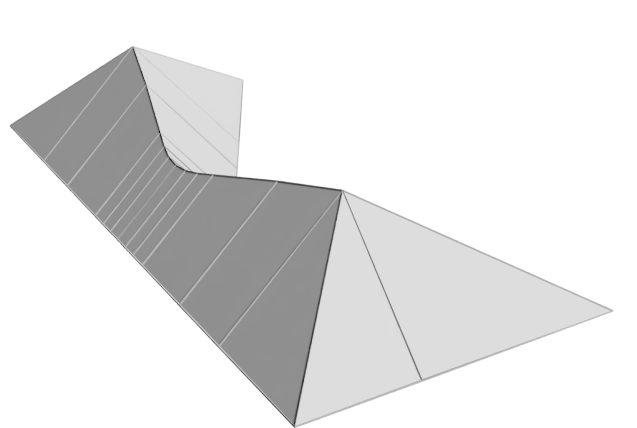
\includegraphics[width=\figwidthTree]{sources/method/surface/union_of_cones_cropped.png}

\vspace{\tempheight}

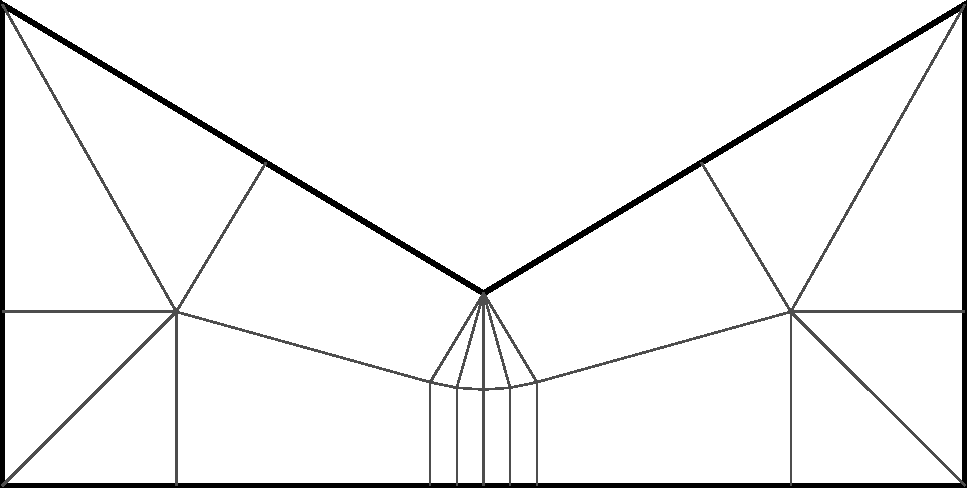
\includegraphics[width=\figwidthTwo]{sources/method/surface/uoc.pdf}
\caption{Union of Cones}\label{3d_surface_overview_uoc}
\end{subfigure}
\begin{subfigure}{\figwidth}\centering
\hspace*{\tempheightTwo}
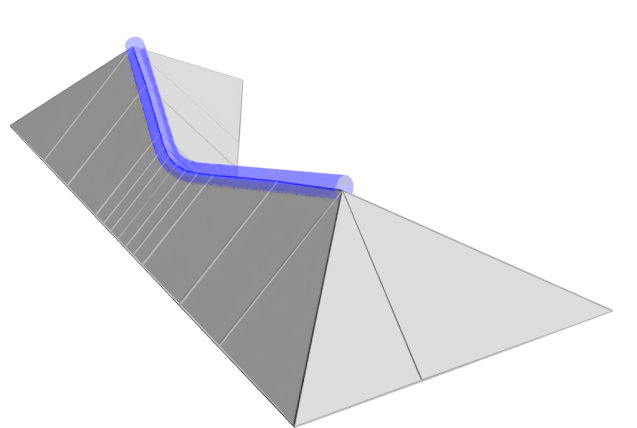
\includegraphics[width=\figwidthTree]{sources/method/surface/marking_cropped.png}

\vspace{\tempheight}

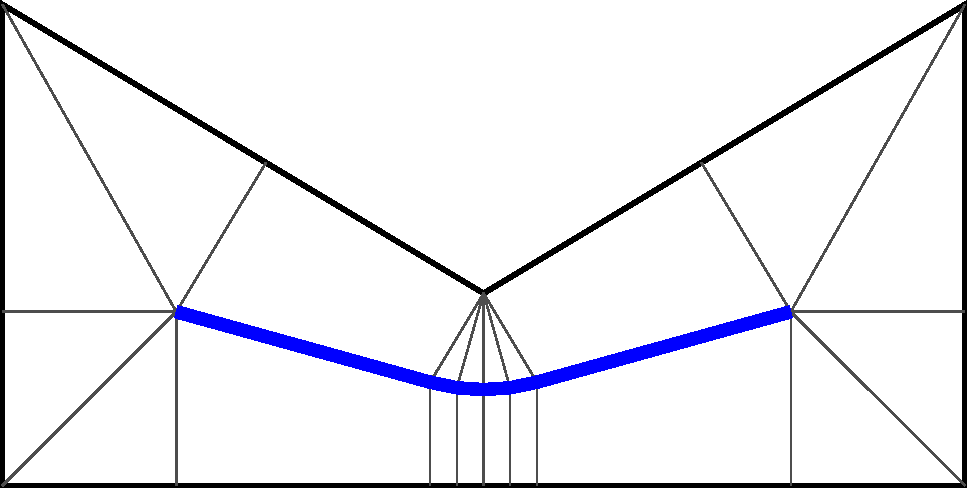
\includegraphics[width=\figwidthTwo]{sources/method/surface/marked.pdf}
\caption{Center}\label{3d_surface_overview_center}
\end{subfigure}
\begin{subfigure}{\figwidth}\centering
\hspace*{\tempheightTwo}
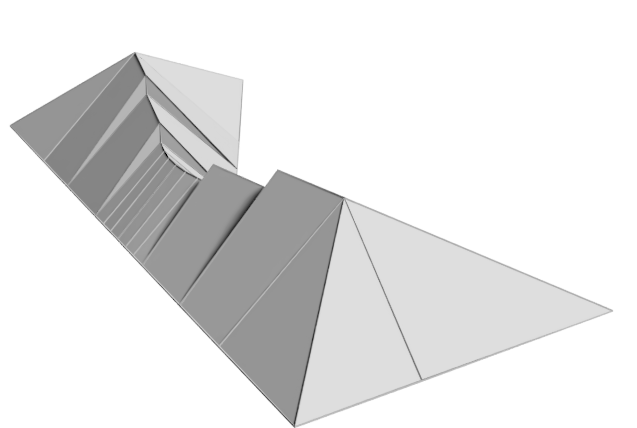
\includegraphics[width=\figwidthTree]{sources/method/surface/rounded_cropped.png}

\vspace{\tempheight}

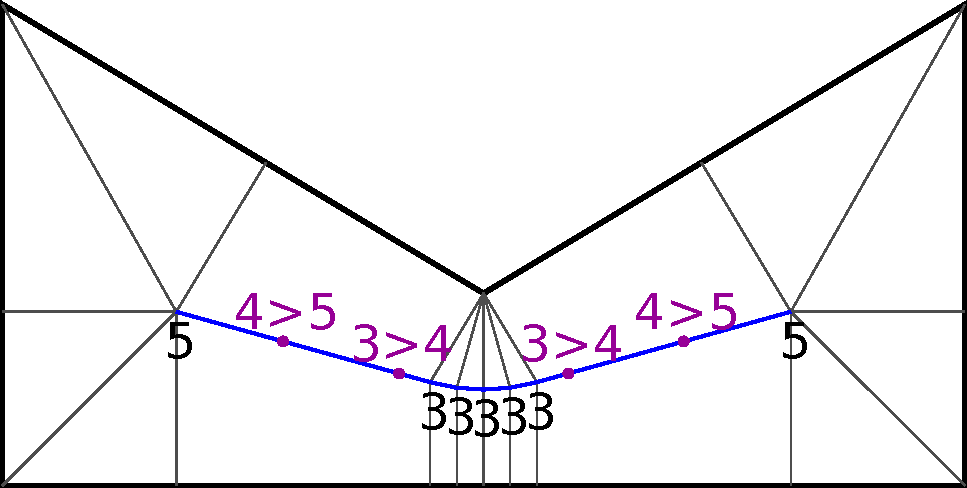
\includegraphics[width=\figwidthTwo]{sources/method/surface/rounded.pdf}
\caption{Flattened}\label{3d_surface_overview_rounded}
\end{subfigure}
\begin{subfigure}{\figwidth}\centering
\hspace*{\tempheightTwo}
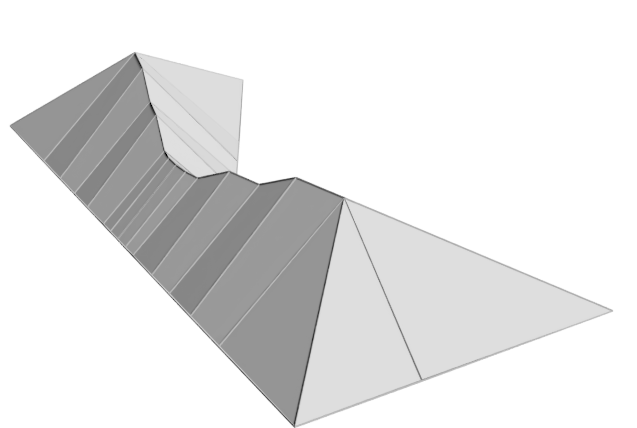
\includegraphics[width=\figwidthTree]{sources/method/surface/smoothed_cropped.png}

\vspace{\tempheight}

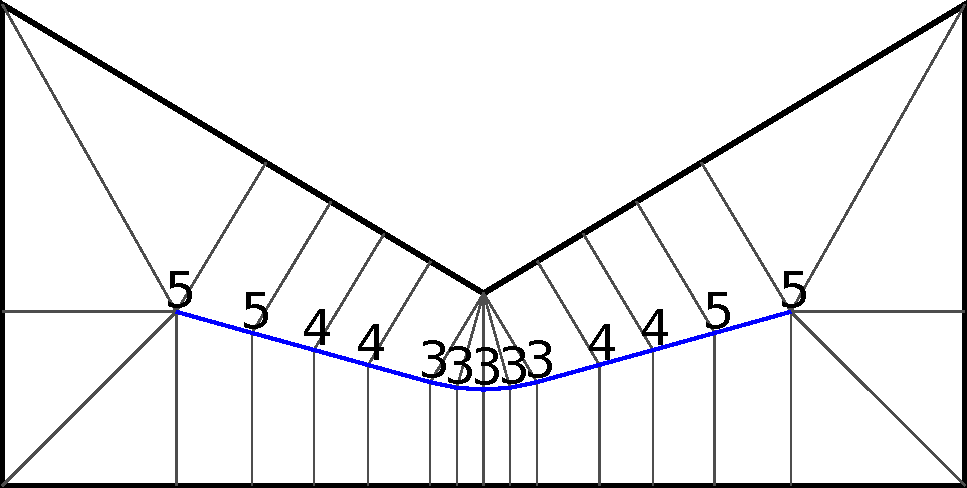
\includegraphics[width=\figwidthTwo]{sources/method/surface/smoothed.pdf}
\caption{Smoothed}\label{3d_surface_overview_smoothed}
\end{subfigure}
\begin{subfigure}{\figwidth}\centering
\hspace*{\tempheightTwo}
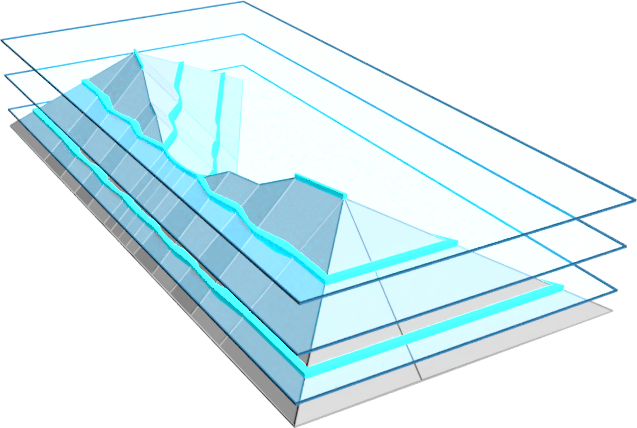
\includegraphics[width=\figwidthTree]{sources/method/surface/sliced_cropped.png}

\vspace{\tempheight}

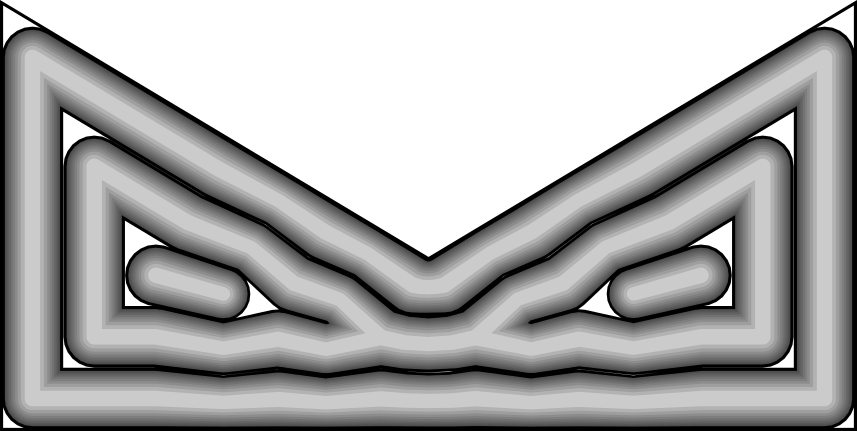
\includegraphics[width=\figwidthTwo]{sources/method/surface/sliced_2D.png}
\caption{Sliced}\label{3d_surface_overview_sliced}
\end{subfigure}
\caption{
A geometrical conceptualization of our technique.
3D visualization on top and the corresponding 2D visualization on bottom.
In the UoC \subref{3d_surface_overview_uoc}
we mark the central regions \subref{3d_surface_overview_center}
and flatten those regions to heights of the nearest integer \subref{3d_surface_overview_rounded}.
We then smooth out the jumps between different integer multiples \subref{3d_surface_overview_smoothed}
and finally we slice the structure to get the toolpaths \subref{3d_surface_overview_sliced}.
Blue signifies regions marked as being central.
The numbers are the integer multiples of half the nozzle width.
}
\label{3d_surface_overview}
\end{figure*}

This section explains how we can generate toolpaths with evenly distributed bead widths.
We describe how to construct the mesh of the UoC in \cref{sec_surface_construction} and
explain how to identify central regions in \cref{sec_center_classification}.
Flattening the central mesh regions and smoothing are handled in \cref{sec_central_height_adjustment}.
We then describe how to deal with heights in the periphery in \cref{sec_peripheral_height_adjustment}
and describe the toolpath extraction algorithm in \cref{sec_toolpath_extraction}.
In \cref{sec_generalization} we describe how to generalize our method for generating evenly distributed bead widths into a general framework for generating contour parallel toolpaths using an arbitrary beading strategy and we show several such beading strategies.


For ease of reference we have included a legend explaining the vocabulary employed in this manuscript in \cref{legend}.

\begin{figure}\centering
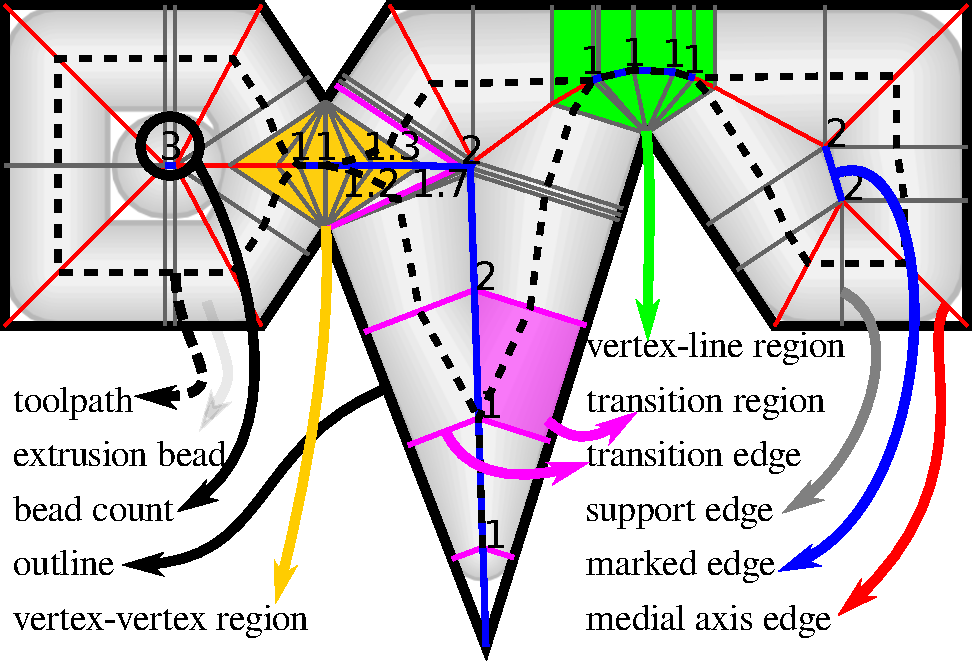
\includegraphics[width=.75\columnwidth]{sources/method/legend2.pdf}
\caption{Explanation of terms and common color coding.}
\label{legend}
\end{figure}








\iffalse

\begin{figure*}
\centering
\setlength{\figwidth}{0.19\textwidth}
\begin{subfigure}{\figwidth}
\centering
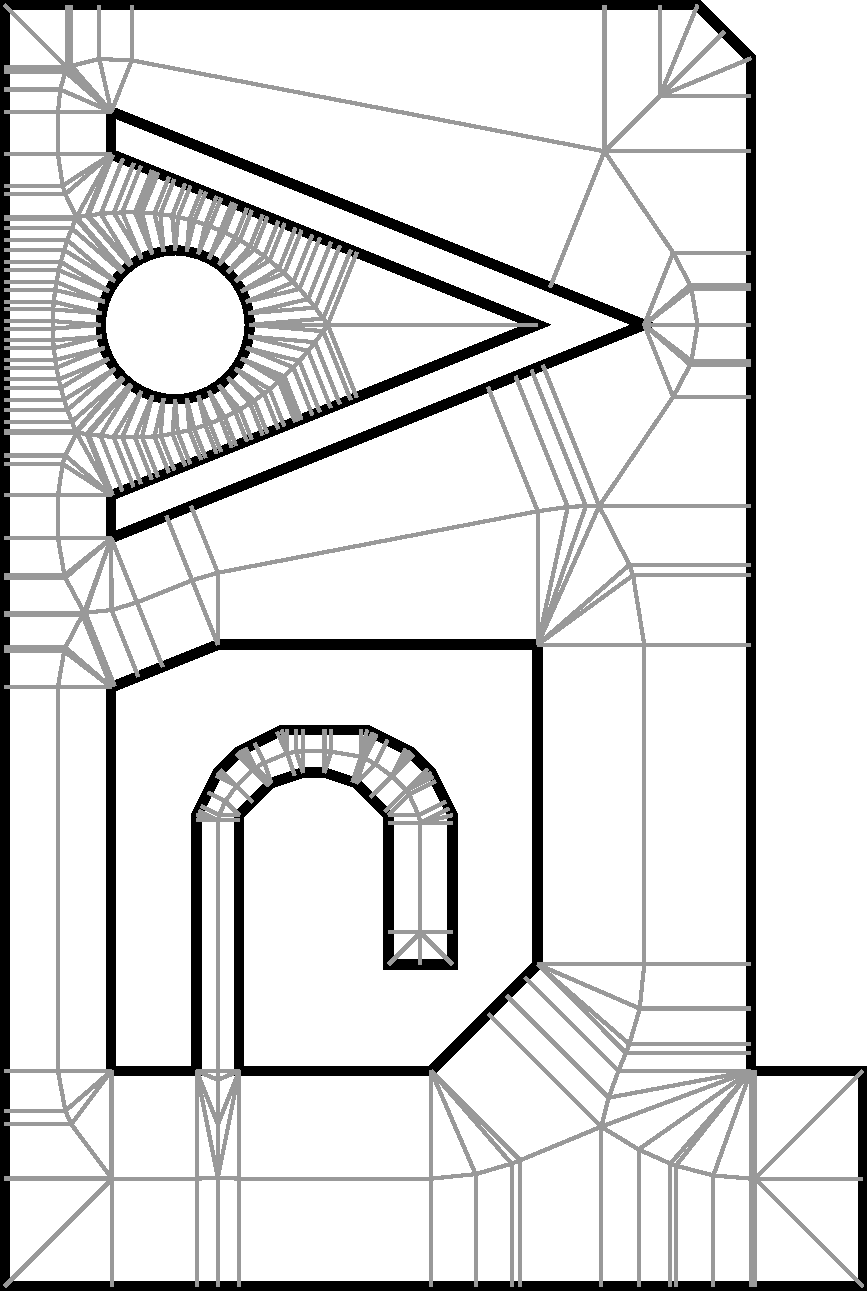
\includegraphics[width=\columnwidth]{sources/method/overview/skeleton.pdf}
\caption{Skeleton}\label{overview_fig_skeleton}
\end{subfigure}
\begin{subfigure}{\figwidth}
\centering
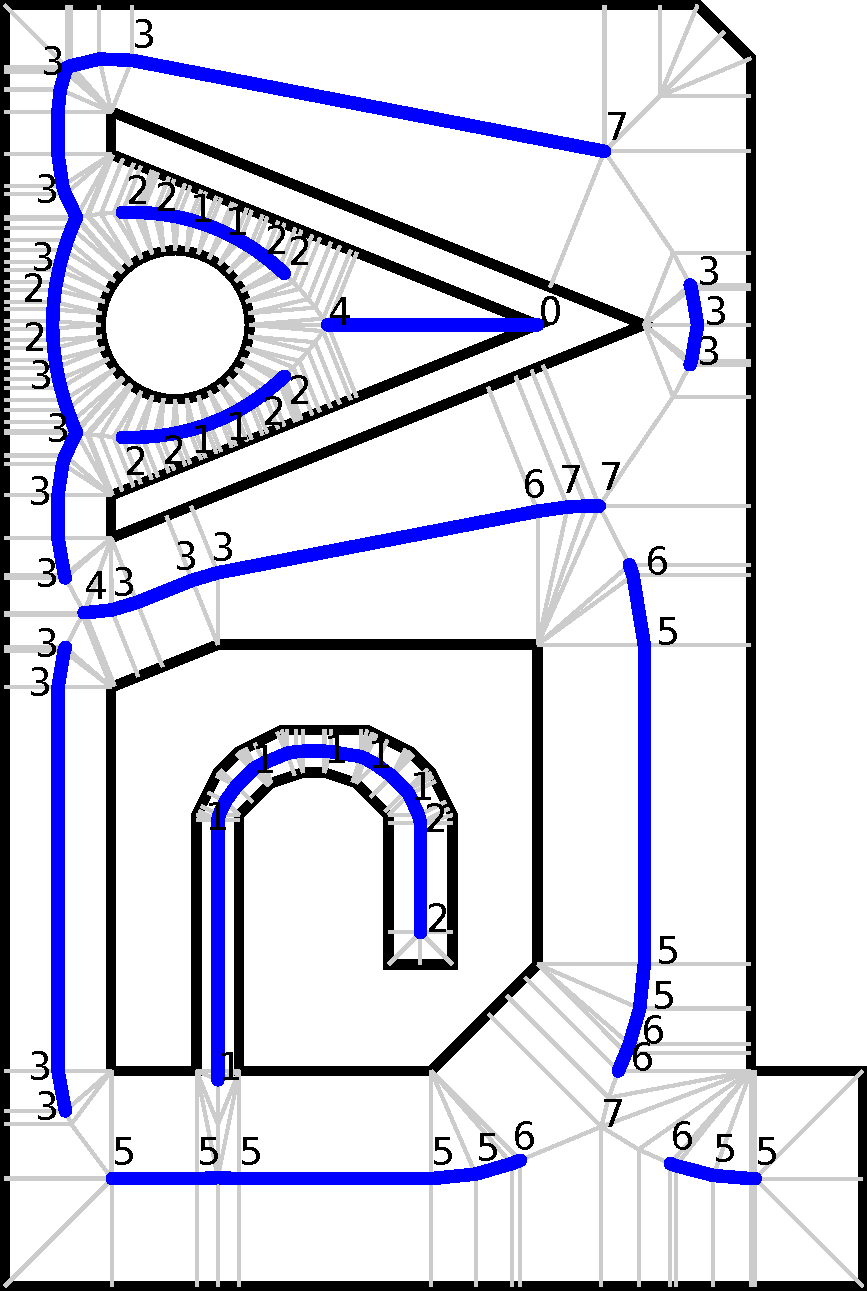
\includegraphics[width=\columnwidth]{sources/method/overview/marked.pdf}
\caption{Marked}\label{overview_fig_marked}
\end{subfigure}
\begin{subfigure}{\figwidth}
\centering
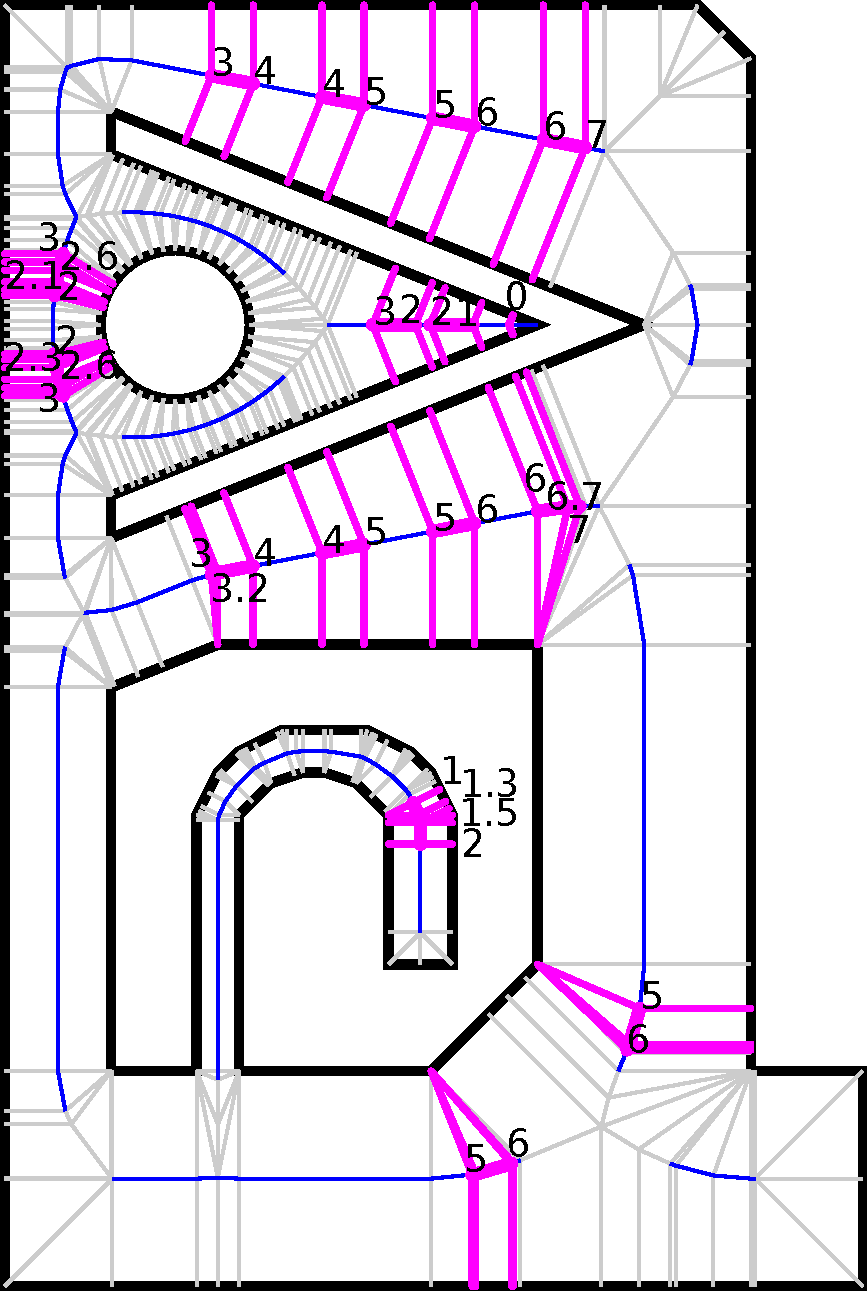
\includegraphics[width=\columnwidth]{sources/method/overview/transitions.pdf}
\caption{Transitions}\label{overview_fig_transitions}
\end{subfigure}
\begin{subfigure}{\figwidth}
\centering
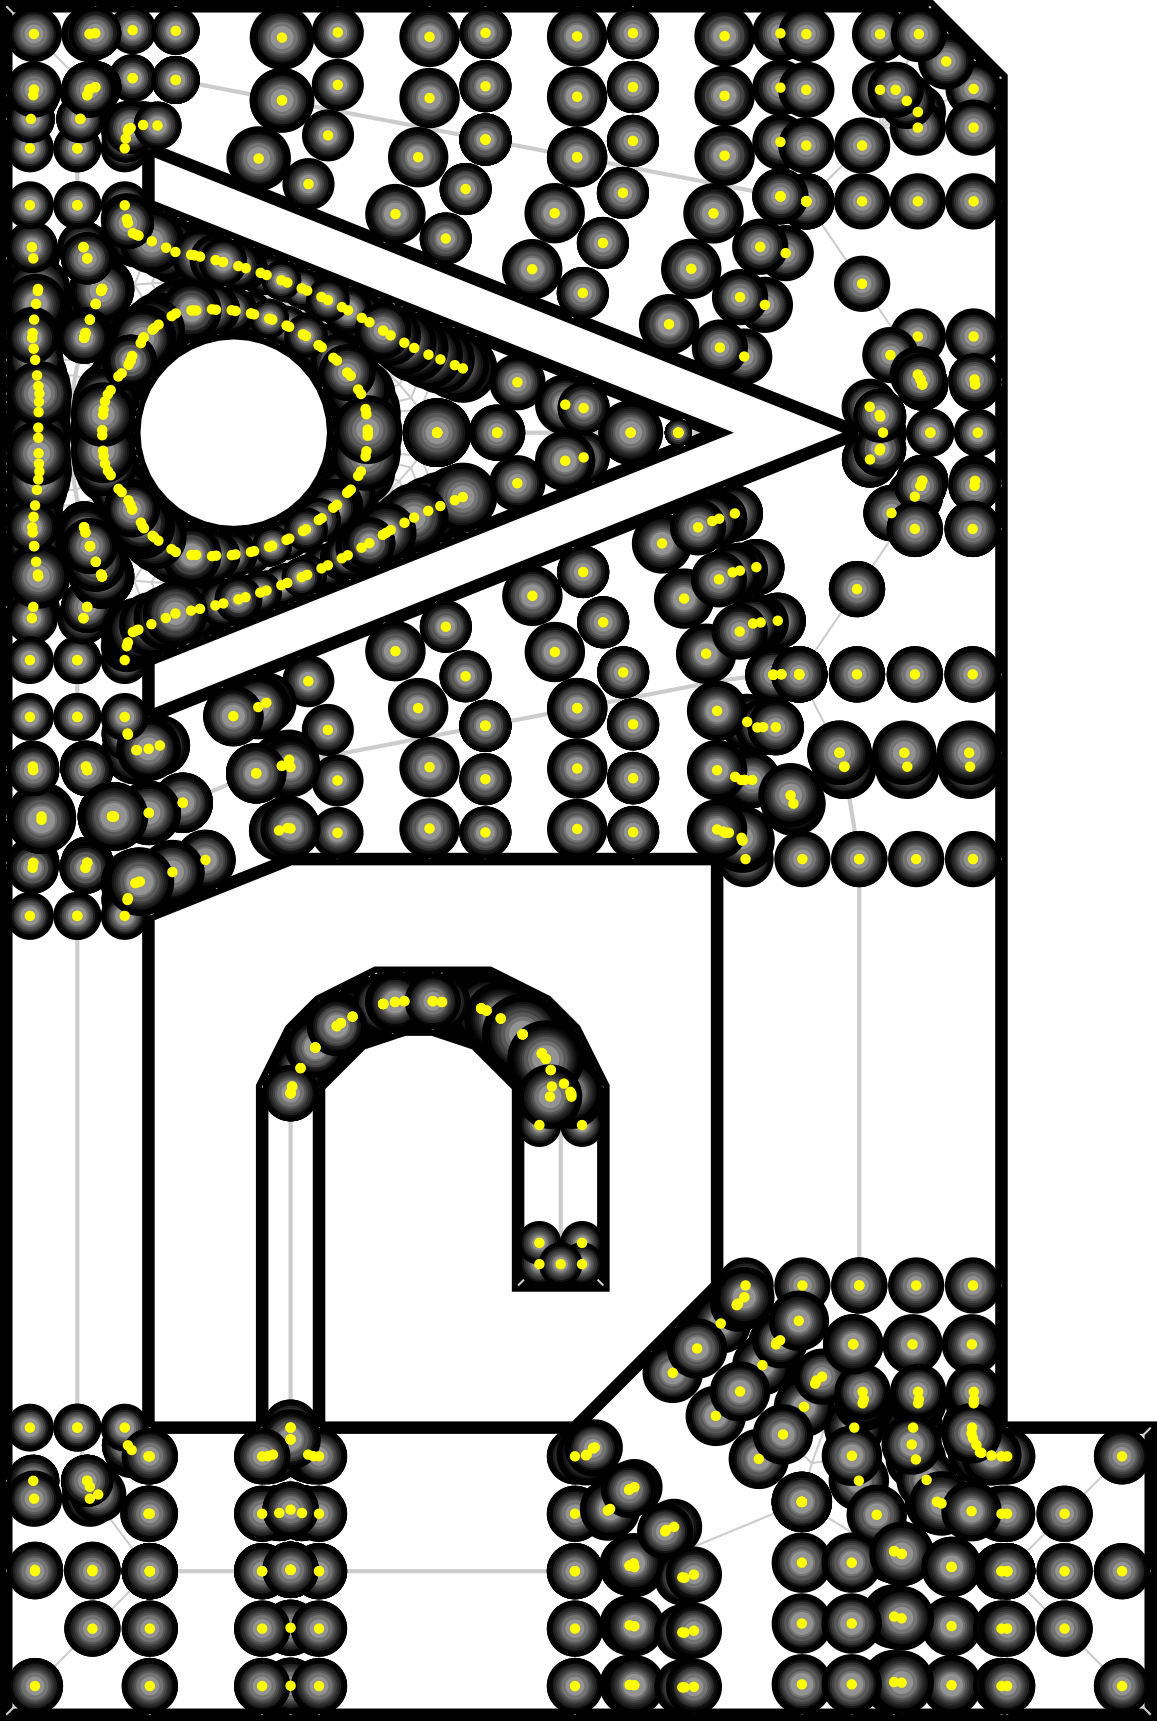
\includegraphics[width=\columnwidth]{sources/method/overview/junctions.png}
\caption{Junctions}\label{overview_fig_junctions}
\end{subfigure}
\begin{subfigure}{\figwidth}
\centering
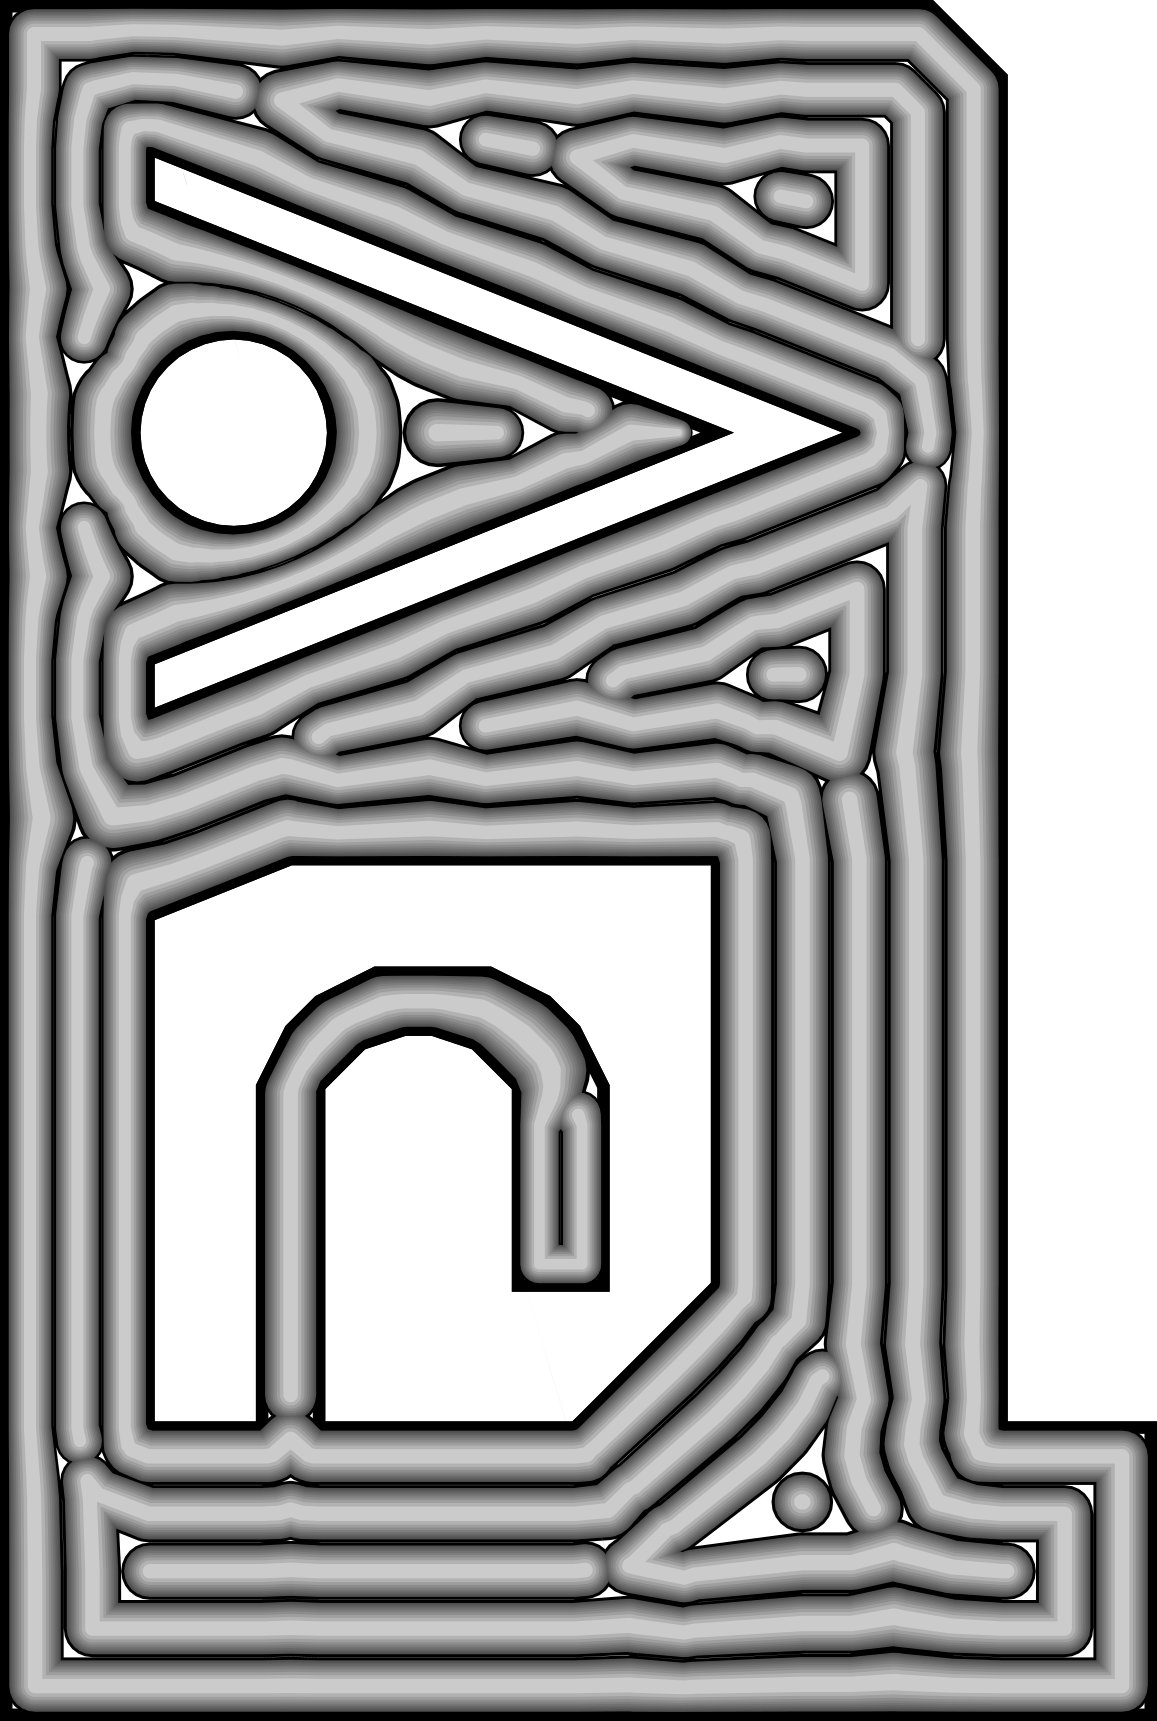
\includegraphics[width=\columnwidth]{sources/method/overview/toolpaths.png}
\caption{Toolpaths}\label{overview_fig_toolpaths}
\end{subfigure}
\caption{
Overview of the steps in the method of our framework.
First we \subref{overview_fig_skeleton} decompose the outline shape into a skeleton (grey), \subref{overview_fig_marked} mark central regions (blue) and determine a bead count (numbers) based on the local feature size.
Then we \subref{overview_fig_transitions} make alterations to smoothly transition to a different bead count (magenta).
We then \subref{overview_fig_junctions} generate a number of junctions (yellow) equal to the bead count along the bones of the skeleton,
which are \subref{overview_fig_toolpaths} connected together to make the toolpaths.
}
\label{overview_fig}
\end{figure*}

\fi














\subsection{Surface generation}\label{sec_surface_construction}
The union of cones surface mesh can be derived from a common skeletonization of the polygonal outline shape: the medial axis.
By assigning each node in the skeleton a height equal to the radial distance to the outline we obtain the shape of the UoC.
Starting from the medial axis we further decompose the shape into simple fragments, so that the mesh contains only quads and triangles.



\subsubsection{Medial axis transform}
One of the most commonly used skeletonizations of a shape is the medial axis.
The medial axis is defined by the locations where the inscribed circle meets the boundary in at least two locations. \cite{blum1967transformation}
We call the set of closest points on the outline polygon $P$ of a point $v$ on the skeleton its \emph{support}: $\text{sup}(v) = \argmin_{x\in P} |x - v|$.
The resulting skeleton consists of straight segments and parabolic segments which form a graph.
See \cref{MAT_explanation_circles}.

Alternatively the medial axis can be defined as the locations where the UoC surface is discontinuous,
or it can be defined as the locations where wave-front propagating from the outline shape make sharp corners. \cite{blum1967transformation}
This last conceptualization is especially relevant because the naive toolpath generation method consists precisely in equidistant wave-fronts from the outline.
The medial axis can therefore be seen as the space within which contour following toolpaths are generated.
See \cref{MAT_explanation}.

%``Because of its shape, the medial axis of a figure is also called the skeleton or the symmetric axis of the figure.'' \cite{lee1982medial} 
``Associated with the medial axis is a radius function $R$, which defines for each point on the axis its distance to the boundary of the object.'' \cite{lee1982medial}
The medial axis along with the feature radius values along the skeleton combine into a complete shape descriptor, called the medial axis transform (MAT).
Feature radius and node locations of segments will be used below to analyse the shape locally.

%\cite{Moesen2011} provides a thorough overview of all MAT algorithms.
%\cite{Moesen2011} calls $R$ the `feature radius': ``In every point $p \in P$, and thus also in points on the MA, the feature radius $\text{rad}(p)$ of $p$ can be defined as the Euclidean distance to the closest point on the boundary of $P$.''


\begin{figure}
\centering
\begin{subfigure}{0.3\columnwidth}
\centering
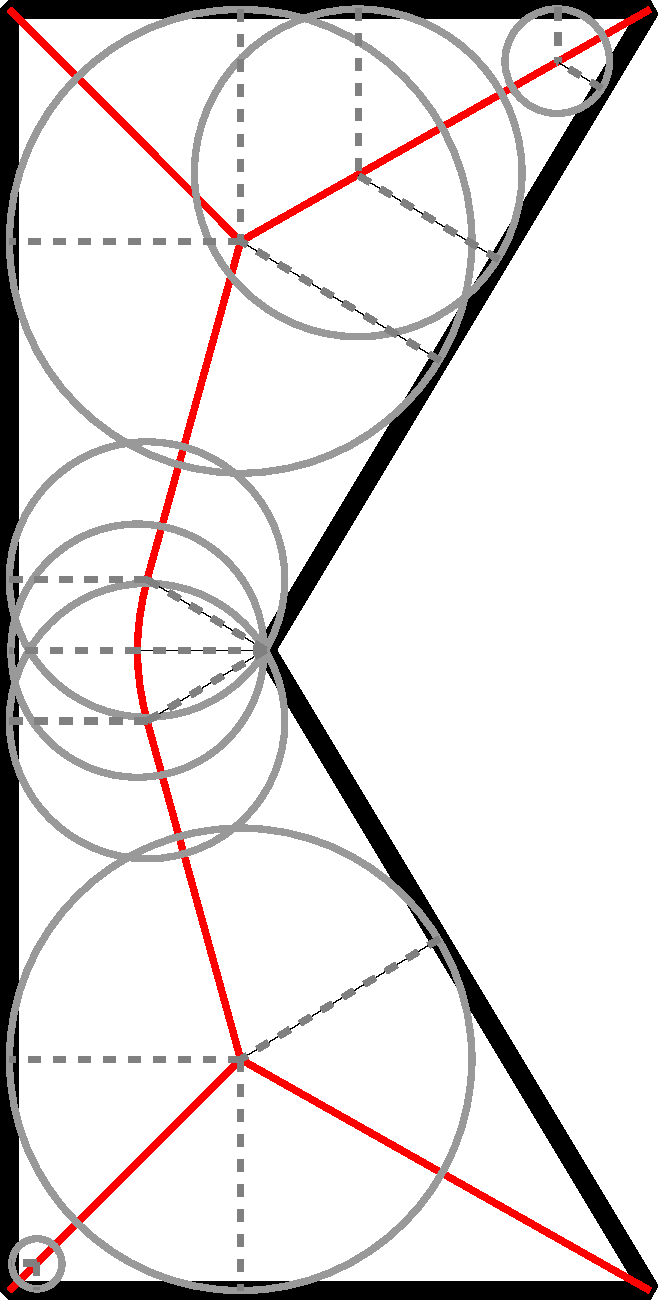
\includegraphics[height=1.5\columnwidth]{sources/method/MAT_explanation_circles.pdf}
\caption{Circles}
\label{MAT_explanation_circles}
\end{subfigure}
\begin{subfigure}{0.3\columnwidth}
\centering
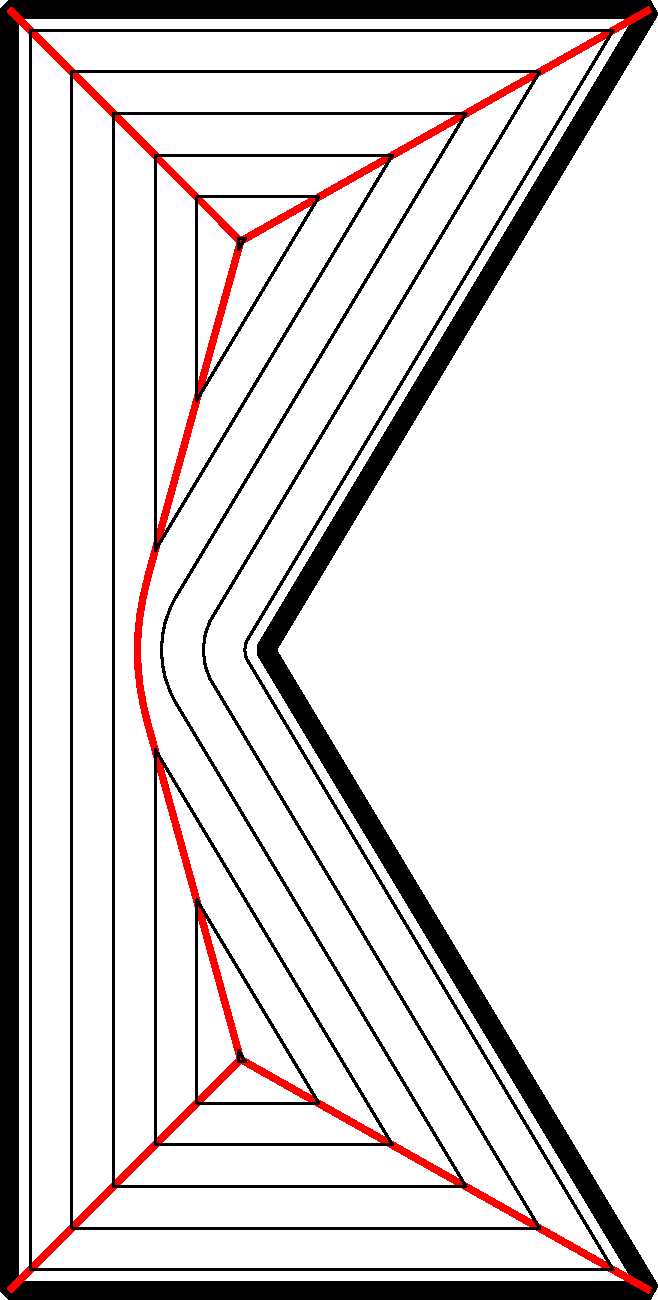
\includegraphics[height=1.5\columnwidth]{sources/method/MAT_explanation_wavefronts.pdf}
\caption{Wave-fronts}
\end{subfigure}
\begin{subfigure}{0.3\columnwidth}
\centering
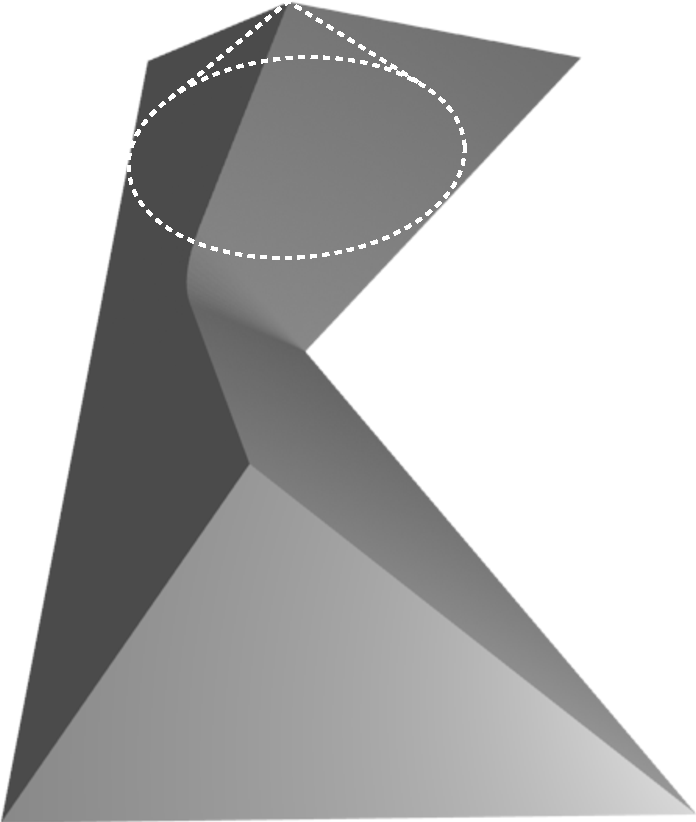
\includegraphics[height=1.5\columnwidth]{sources/method/MAT_explanation_cones.pdf}
\caption{Union of Cones}
\end{subfigure}
\caption{
Medial axis representations.
The medial axis can be defined in terms of the the number of support points of the inscribed circles,
as the pinch sites in wave-fronts
or as ridges in a volume defined by the union of cones.
}
\label{MAT_explanation}
\end{figure}


\begin{figure}\centering
\setlength{\figwidth}{0.19\columnwidth}
\setlength{\figwidthTwo}{0.3\columnwidth}
\begin{subfigure}{\figwidth}\centering
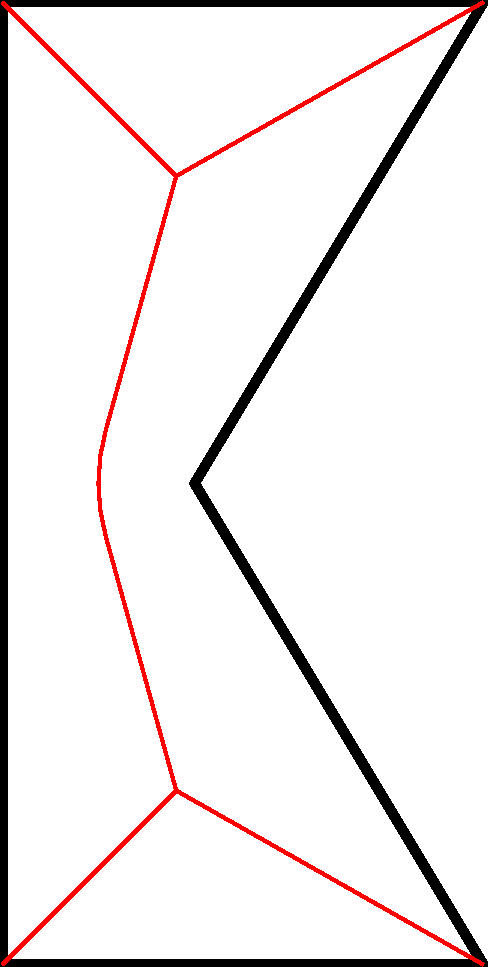
\includegraphics[height=\figwidthTwo]{sources/method/simple_skeleton_mat}
\caption{Medial Axis}\label{shape_decomposition_mat}
\end{subfigure}
\begin{subfigure}{\figwidth}\centering
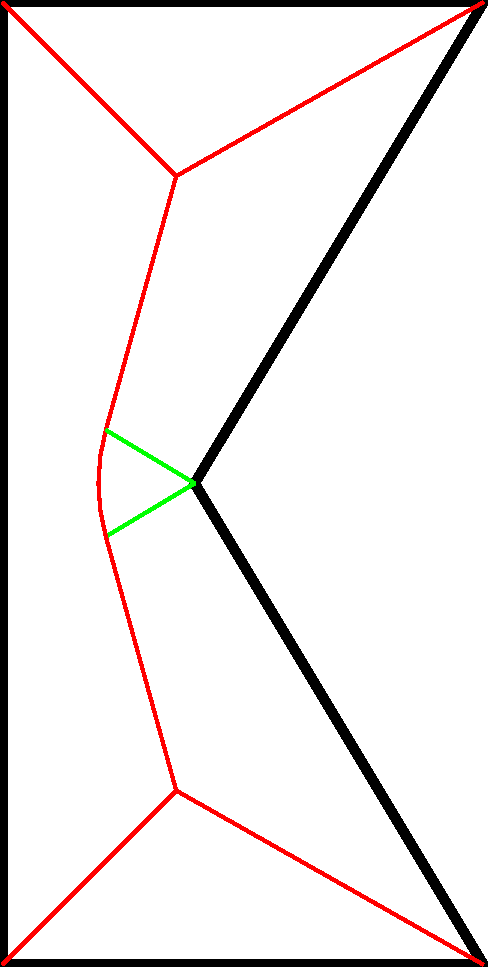
\includegraphics[height=\figwidthTwo]{sources/method/simple_skeleton_vd}
\caption{Voronoi Diagram}\label{shape_decomposition_vd}
\end{subfigure}
\begin{subfigure}{\figwidth}\centering
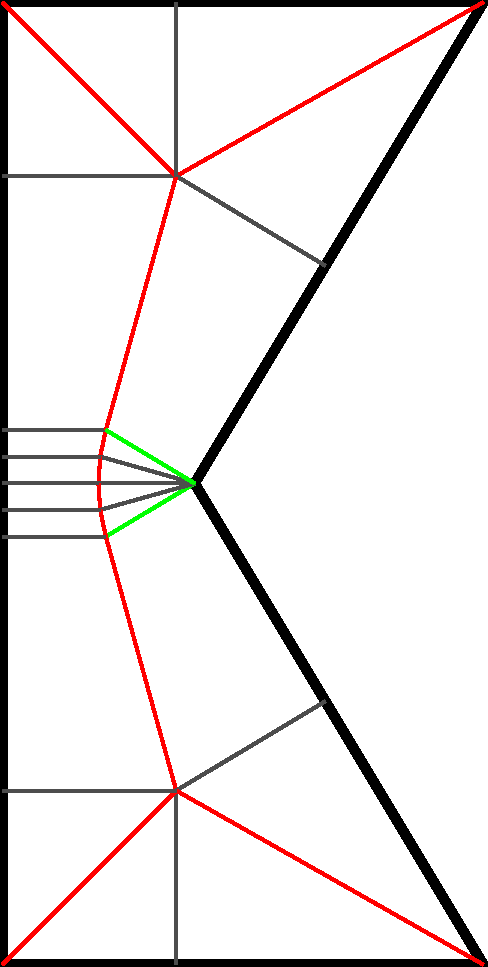
\includegraphics[height=\figwidthTwo]{sources/method/simple_skeleton_st}
\caption{Skeletal Trapezoids}\label{shape_decomposition_st}
\end{subfigure}
\begin{subfigure}{\figwidth}\centering
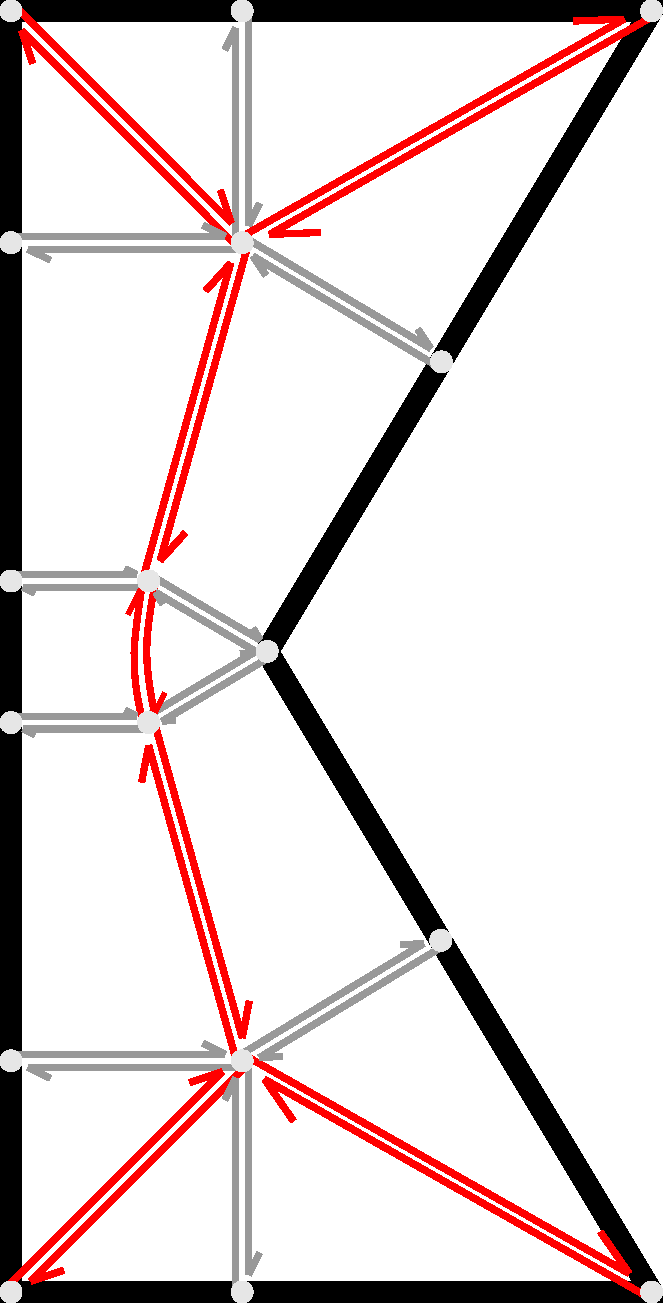
\includegraphics[height=\figwidthTwo]{sources/method/half_edge_datastructure.pdf}
\caption{Data structure}\label{shape_decomposition_datastructure}
\end{subfigure}
\begin{subfigure}{\figwidth}\centering
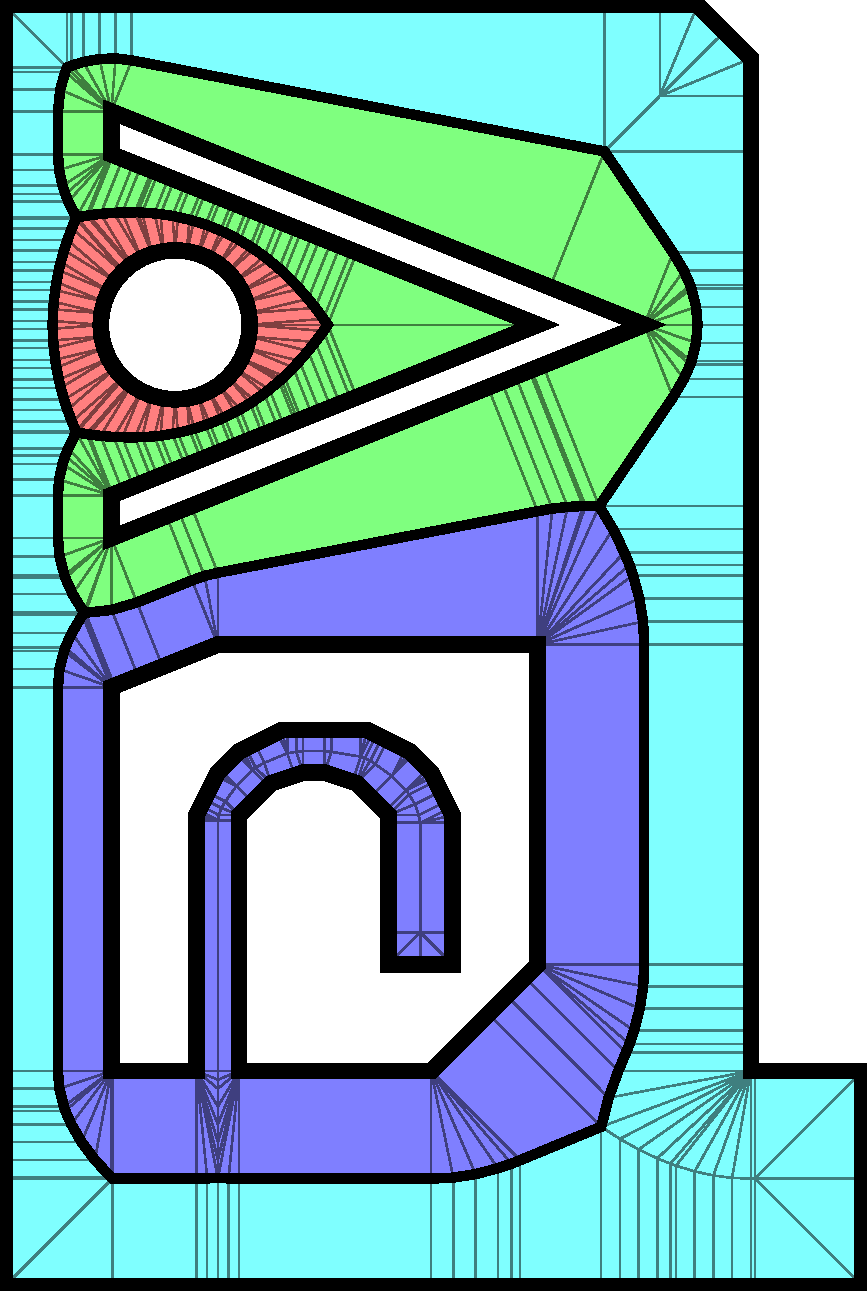
\includegraphics[height=\figwidthTwo]{sources/method/domains.pdf}
\caption{Polygon Domains}\label{shape_decomposition_domains}
\end{subfigure}
\caption{
Skeletonization of an outline shape (black).
Relation between the medial axis (red), the limited Voronoi Diagram (red and green) and the Skeletal Trapezoidation (red, green and gray): MAT $\subset$ Limited VD $\subset$ ST.
}
\label{skeletonization_comparison}
\end{figure}



\subsubsection{Skeletal trapezoidation}
The MAT decomposes the outline shape into several complex shapes which we need to further decompose in order to have a mesh consisting only of quads and triangles.
We employ a shape decomposition proposed by \citeauthor{Ding2016a}. \cite{Ding2016a}
Each of the regions demarcated by the skeleton is further decomposed by adding radial bones from each node $v$ to its support $\text{sup}(v)$.
The resulting skeleton decomposes the outline shape into trapezoids and triangles.
We will therefore call this shape decomposition the \emph{Skeletal Trapezoidation} (ST).
(The concept of a trapezoidation conventionally allows for the degenerate case where a trapezoid resolves into a triangle. \cite{chazelle1984,fournier1984})
We represent such a skeleton in a standard half-edge data-structure.
See \cref{shape_decomposition_datastructure}.

The trapezoids are classified as belonging to a specific domain following \citeauthor{Ding2016a}.
Each polygon in the input shape acquires it's own domain.
The domains of hole polygons are touching the domains of the outer polygon.
See \cref{shape_decomposition_domains}.


The medial axis of a polygonal shape can be obtained from the Voronoi Diagram (VD) generated on the line segments and vertices of the shape, by throwing away all segments of the VD falling outside of the outline shape and throwing away the bones connected to concave vertices in the outline shape. \cite{lee1982medial}
However, the concave vertices are precisely in the support of the nodes to which those bones connect.
This means we can efficiently compute the ST from the VD by removing all segments which lie outside the outline shape and add radial bones to the nodes from there.
See \cref{skeletonization_comparison}.


We then also discretize parabolic segments and segments generated by two concave outline vertices into segments approximately as long as some constant $d^\text{discretization}$.
See \cref{discretization} and the middle of \cref{shape_decomposition_st}.
That way we can approximate the feature radius $R$ in between the two nodes $v_0$ and $v_1$ of a bone in the ST by interpolating linearly between $R(v_0)$ and $R(v_1)$.
This makes the skeleton capture a discrete approximation of the radius function which is then used to determine the height of each node in the skeleton in order to generate the 3D mesh of the UoC.
The UoC is the ST along with the corresponding feature radius $R$ as the height of each node.
%; see \cref{mat_3d}.




\iffalse

\begin{figure}
\centering
%\begin{subfigure}{0.45\textwidth}
%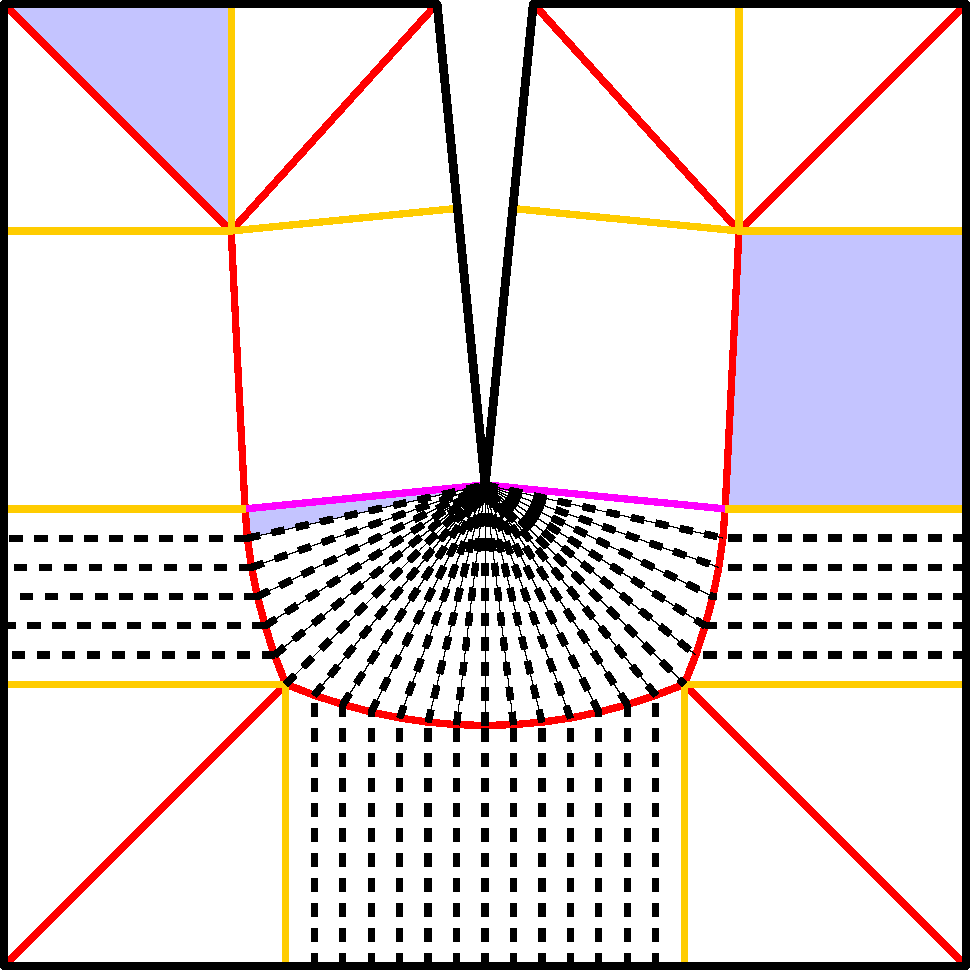
\includegraphics[width=\columnwidth]{sources/method/parabola_dip.pdf}
%\caption{asf}
%\end{subfigure}
%\begin{subfigure}{0.45\textwidth}
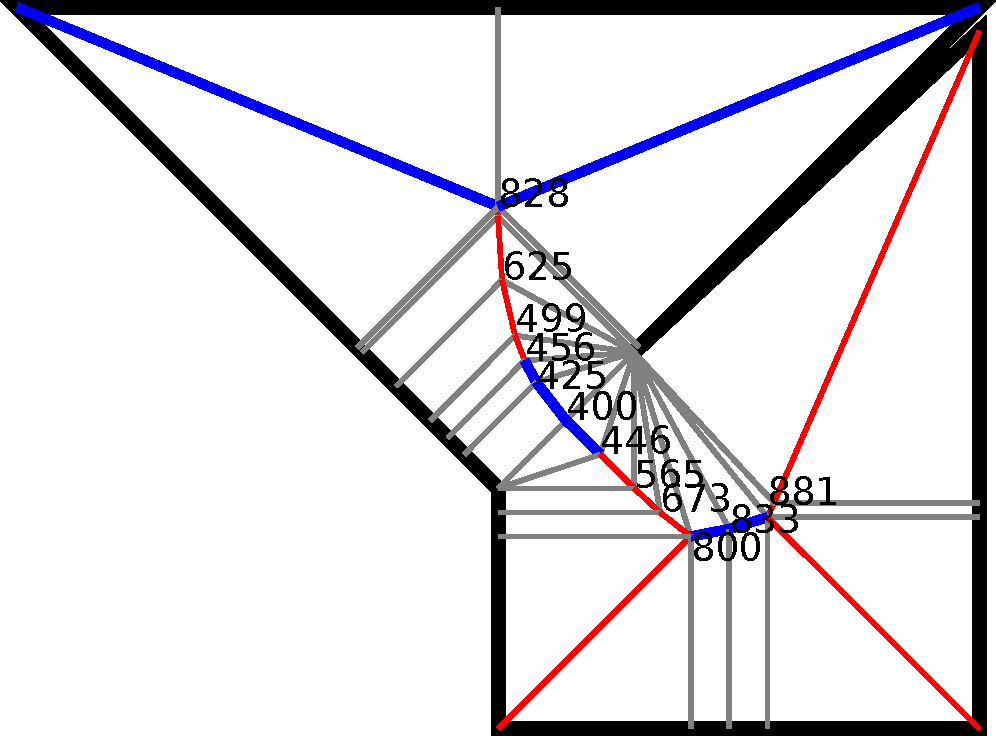
\includegraphics[width=.5\columnwidth]{sources/method/point-point_and_point-line_segments.pdf}
%\caption{Transitioning}
%\end{subfigure}
\caption{
Skeletal trapezoidation domain decomposition.
Medial axis (red and blue) is augmented with (gray) edges connecting each node to its nearest support points in the outline shape.
Parabolic medial axis segments are discretized and likewise for segments generated by two concave outline vertices, because the feature radius (black text in microns) doesn't increase linearly along those segments.
The blue segments are significant according to $\alpha_\text{max} = 135\degree$.
}
\label{discretization}
\end{figure}

\fi



\subsubsection{Union of cones}
In order to transform the ST into a 3D surface we add another dimension to the skeleton.
We assign each node a height value measured in terms of an integer number: it's \emph{bead count}.
We define the bead count as the number of beads to fit along the \emph{diameter} of the shape, which is twice the feature radius.
While the feature radii are measured along the support bones, the diameter is not measurable as such because the support bones are generally not collinear;
we introduce the concept of the diameter so that we can deal with an odd number of beads while using integer logic.

For each node $v$ we assign an initial bead count based on the feature diameter $2R$ and the nozzle size $w_\text{pref}$: $b^*_v \leftarrow 2 R(v) / w_\text{pref}$.
The result is a mesh representing the union of cones (UoC) consisting entirely of quads and triangles.
Note that although the overview of the method was described geometrically in terms of the UoC, the actual method relies on the 2-dimensional ST, while the use of the bead count as a height value is only a visualization aid.















\subsection{Center classification}\label{sec_center_classification}
The naive method of performing constant width offset produces large overfill and underfill areas on central regions of the skeleton.
These central regions present themselves as upper ridges in the mountains of the UoC surface.
This sections covers what parts of the UoC will be marked as being central, rather than peripheral.

We mark a node of the skeleton as central if its feature radius is larger than that of all of the neighboring nodes in the skeletal graph.
That is: we mark the local maxima, i.e. the mountain tops of the UoC as being central.
We also mark whole bones as being central if they are significant according to a significance measure which is commonly used in shape analysis.


\subsubsection{Significance measure}\label{sec:significance_measure}
Centrality can be formalized by looking at a commonly used significance measure knows as the \emph{bisector angle}.
The bisector angle $\alpha$ is the interior angle $\angle{p_ovp_1} \leq \si{180}{\degree}$ between a location $v$ on a bone of the skeleton and its two supporting polygon points $p_0$ and $p_1$.\cite{attali1996modeling}
Bones are significant if the bisector angle exceeds $\alpha_\text{max}$ which is governed by the beading strategy.

For a polygon with a pointy wedge area of an angle $\beta$, we have $\alpha = 180\degree - \beta$, which corresponds to overfill areas and underfill areas the size of $\nicefrac12 w^2 \left( \nicefrac14 \tan ( \alpha / 2) - \alpha / 2 \right)$ when filled using a naive strategy of constant bead width $w$.
See \cref{naive_overfill_underfill}.
The bisector angle is therefore an exact measure of the amount of overfill and underfill in the naive toolpaths of constant width.
%Contrary to related literature we will \emph{keep} the non-significant regions of the skeleton.
We mark all significant bones as such and contrary to related literature we keep the unmarked bones of the skeleton.
Our framework will decide on a beading at all of the marked nodes in `the center' nodes and apply the beading outward to the unmarked nodes.


\begin{figure}
\centering
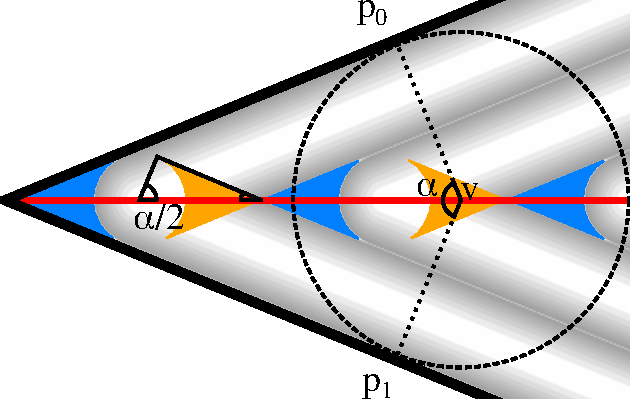
\includegraphics[width=.5\columnwidth]{sources/method/naive_overfill_underfill.pdf}
\caption{
Overfill and underfill areas in a naive beading using a constant bead width $w$ of a wedge area with vertex angle $\beta$.
The underfill areas (light blue) are mirrored versions of the overfill areas (dark red).
The bisector angle $a = 180\degree - \beta$ is the angle between a location $v$ and its support $p_0$ and $p_1$.
}
\label{naive_overfill_underfill}
\end{figure}


A computationally efficient way to compute whether an edge is significant can be obtained by looking at the ratio between feature radius $R$ and the Euclidean distance:
if $ | R(v_1) - R(v_0) | / |v_1 - v_0| >  \cos(\alpha_\text{max} / 2)$ then $\alpha > \alpha_\text{max}$.
See \cref{distance_based_angles}.
This means we can prevent executing trigonometric functions on \emph{each} of the bones in the skeleton.
Moreover the ratio has a clear geometrical interpretation as the slope of the ridge in the UoC surface.

This ratio can readily be applied to simple skeleton segments to determine whether they are significant.
For skeletal segments generated by a polygon vertex at $(0,d)$ and a line segment through $(0,0)$ and $(0,\epsilon)$ or another vertex $(0,0)$, we can determine the significant portion by evaluating $\frac{\partial R}{\partial x} > \cos(\alpha_\text{max} / 2)$.
For parabolas we introduce extra points in the discretization at the two bounds where $| x | = d  / \tan(\alpha_\text{max} / 2)$
and for bones with vertex-vertex support we introduce discretization points at the two bounds where $| x | = \nicefrac12 d  / \tan(\alpha_\text{max} / 2)$.
This ensures that the discretization doesn't alter the extent and existence of marked central regions.
See \cref{legend}.


\begin{figure} \centering
\newlength{\significancePropertiesHeight}
\setlength{\significancePropertiesHeight}{.25\columnwidth}
\begin{subfigure}{0.35\columnwidth} \centering
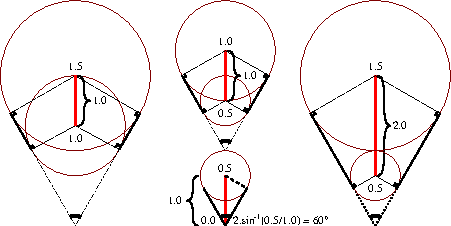
\includegraphics[height=\significancePropertiesHeight]{sources/method/distance_based_angles.pdf}
\caption{Significance}
\label{distance_based_angles}
\end{subfigure}
\begin{subfigure}{0.3\columnwidth} \centering
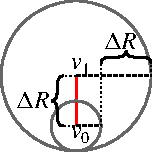
\includegraphics[height=\significancePropertiesHeight]{sources/method/distance_ratio_limit.pdf}
\caption{Distance}
\label{distance_ratio_limit}
\end{subfigure}
\begin{subfigure}{0.3\columnwidth} \centering
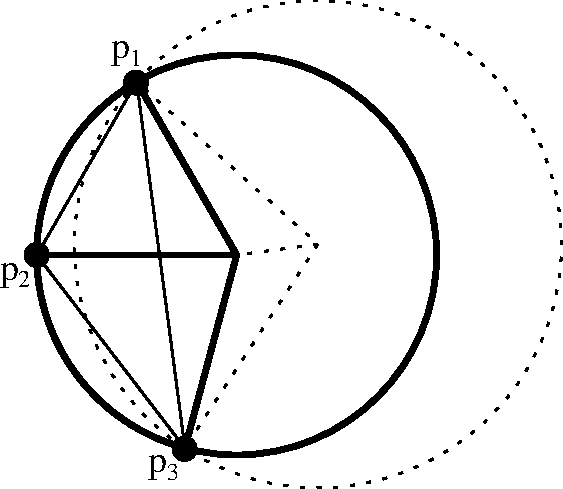
\includegraphics[height=\significancePropertiesHeight]{sources/method/branch_upward_edge_property.pdf}
\caption{Upward edge}
\label{branch_upward_edge_property}
\end{subfigure}
\caption{
Properties of feature radius $R$.
Part of outline shape in thick black,
skeleton in red,
inscribed circle in gray,
radii in dashed lines.
\subref{distance_based_angles} The significance measure can be simplified using $\alpha = 2 \gamma = 2 \cos^{-1} \Delta R / |v_1 - v_0|$.
\subref{distance_ratio_limit} The distance $|v_1 - v_0| > \Delta R$ because otherwise the feature radius would not be one of an inscribed circle.
\subref{branch_upward_edge_property} The radial distance can only increase along one edge around a branch point in the medial axis.
}
\end{figure}




\iffalse

\subsubsection{Properties of significant regions}
%\begin{lemma} \label{min_euclidean_distance} >> this paragraph contains two lemmas and a concluding remark!
The Euclidean distance between two skeletal vertices can never be less than the difference in the feature radius $R$ measure between the vertices.
See \cref{distance_ratio_limit}.
The condition $|v - p| = \Delta R$ is true exactly for those sekeletal bones between a node $v$ and an outline location $p$ added by the trapezoidation, which means that the trapezoidation never introduces marked bones, so we can perform the trapezoidation after marking.


\iffalse
% This fact is not used anymore, because we change the marking such that it doesn't hold for marked edges any more.
A node in the graph can have at most two significant edges.
For a node in the VD $v$ with a support of three points on the outline polygon $p_1, p_2, p_3$, the bisector angles $\angle{p_1vp_2} + \angle{p_2vp_3} + \angle{p_3vp_1} = 360\degree$, so if two angles are more than $\alpha_\text{max} > 120\degree$ the third one needs to be smaller than $360\degree - 2\alpha_\text{max} < 120\degree$ and therefore nonsignificant.
% However, because of some filtering operations this property does not neccesarily hold for the markings.
The extra edges added to the VD to form the ST can never be significant because their bisector angle is \SI{0}{\degree} by definition,
so the nodes of the ST also have at most two significant edges.
\fi

\begin{lemma}\label{saddle_points_are_marked}
A saddle point is always marked, i.e.\
when traversing the skeletal graph from one locally maximal $R$ to another we must pass through a significant region.
\end{lemma}
\begin{proof}
You will either go through the marked region of a discretized parabola or of a segment with two polygonal vertices as support.
This means that the feature radius function in between marked regions is always monotonic.
This means that when propagating beadings downward from marked regions they can never conflict in the middle - they will always conflict at either marked region.
\end{proof}

\begin{lemma}\label{single_upward_edge}
From any node in the graph which is not a saddle point there is at most a single edge going upward.
\end{lemma}
\begin{proof}
Any branch point $v$ in the MAT coincides with the circumcircle of its support $p_0, p_1, p_2$.
If $v$ lies within $\triangle p_0 p_1 p_2$ it is a local maximum and otherwise we will show it has exactly one upward edge.
If $v$ lies outside of $\triangle p_0 p_1 p_2$ then those support points lie within a \SI{180}{\degree} range from $v$
and one point lies in the middle, say $\angle p_0 + \angle p_1 = \angle p_2$.
Then a circle with radius $R(v) + \epsilon$ around $v'$ such that $|v-v'| < \epsilon$ can only touch $p_0$ and $p_2$.
See \cref{branch_upward_edge_property}.
%See VoronoiQuadrangulation::filterUnmarkedRegions
Bones added because of the trapezoidation always go down to $R=0$, so these don't change the property that each node has at most a single upward edge.
This means that walking up the graph from a marked region to a local maximum follows a single path without branching.
\end{proof}

\fi


\iffalse
% This fact is not used anymore, because we change the marking such that it doesn't hold for marked edges any more.
The two downward edges from a branch point cannot both be significant.
A branch point which is not a local maximum generated by the support points $p_1, p_2, p_3$ has bisector angles such that $\triangle p_1 p_2 p_3$ has its circumcentre $v$ outside of the triangle, because otherwise the feature radius decreases in all directions.
This means that all support points lie within a \SI{180}{\degree} range around the node. 
Suppose the one edge going upward is generated by $p_1$ and $p_3$.
Then the bisector angle $\angle p_1 v p_3 < 180\degree$ and $\angle p_1 v p_2 + \angle p_2 v p_3 < 180\degree$,
so if $\angle p_1 v p_2 < 120\degree$ then $\angle p_2 v p_3 < 60\degree$ and is therefore not significant. 
%so at most either of $\angle p_1 v p_2$ and $\angle p_2 v p_3$ has a significant bisector angle.
\fi



\subsubsection{Marking filtering}
Using the significance measure and the local maximum feature radius condition we initialize all marked bones and nodes.
We then filter out high frequency changes in the marking in order to ensure that the output of our technique is smooth. 
We perform filtering on the unmarked regions, because unmarking central regions could reintroduce large over- and underfill areas.
From each marked node $v_0$ with an upward unmarked bone attached we walk along the upward edges;
if the total length traversed until we reach another marked node $v_1$ is shorter than some filter distance $d_\text{max}^\text{unmarked}$, we mark all bones encountered as being central.















\subsection{Central height adjustment}\label{sec_central_height_adjustment}
Now that we have identified and marked the central regions we flatten those regions to integer heights.
More specifically we round the heights to integer bead count values.
When the heights of a ridge are rounded to an \emph{even} bead count, the ridge will be sliced as normal; the intersection between a slicing plane and the mesh surface results in a polyline on both sides of the ridge, which are connected together into a polygonal toolpath.
When the heights of a ridge are rounded to an \emph{odd} bead count, the ridge will coincide exactly with a slicing height, which results in a single polyline toolpath being generated along the middle of the feature.

%\subsubsection{Initial bead count}\label{sec_initial_bead_count}
In order to update the bead count values, we require a flattening operator which maps a feature diameter to a bead count: $f: \mathbb{R} \to \mathbb{N}$.
For our example we choose to round to the nearest integer multiple of the nozzle size $w_\text{pref}$: $f(d) = \left\lfloor \nicefrac{d}{w_\text{pref}} + \nicefrac12 \right\rfloor$.
In our generalized framewotk the function $b$ is determined by a beading strategy.

We first assign each marked node $v$ of the skeleton the bead count $b^*_v \leftarrow f(2R(v))$.
We then filter out short unmarked regions where the bead count remains constant in order to limit the extent of a problem handled in \cref{section_beading_conflicts}.
From each marked node $v_0$ with an upward unmarked bone attached we walk along the upward edges until we hit another marked node $v_1$.
If the upper node has the same bead count $b^*_{v_1} = b^*_{v_0}$ we mark all bones and nodes $v$ in between, and set the bead count $b^*_v \leftarrow b^*_{v_0}$.


\begin{figure*}
\centering
\setlength{\figwidth}{0.13\textwidth}
\begin{subfigure}{\figwidth}
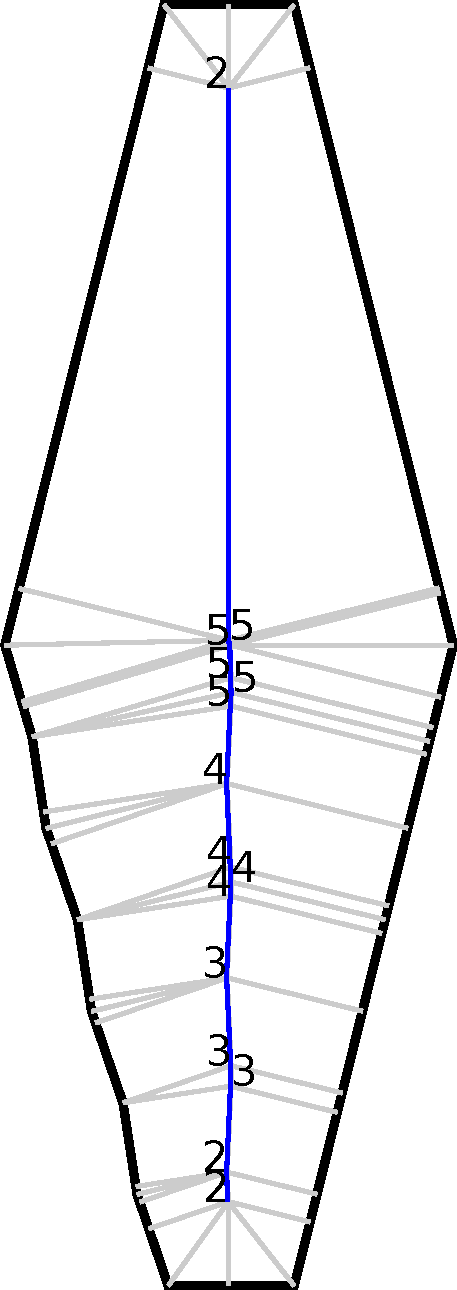
\includegraphics[width=\columnwidth]{sources/method/beading_transitioning_filtering__bead_count.pdf}
\caption{Flattened bead counts}\label{beading_transitioning_filtering__bead_count}
\end{subfigure}
\begin{subfigure}{\figwidth}
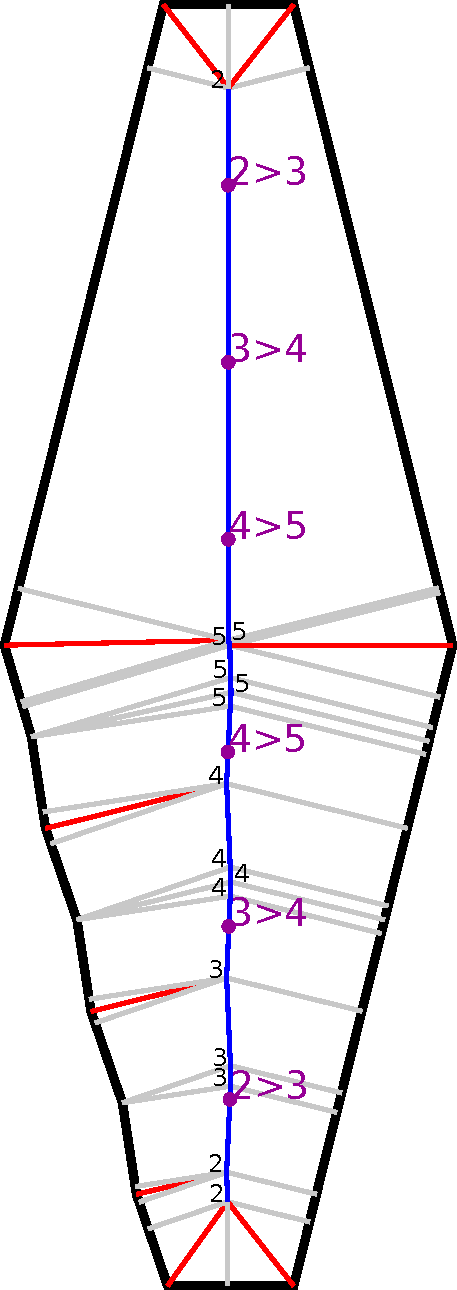
\includegraphics[width=\columnwidth]{sources/method/beading_transitioning_filtering__transition_mids.pdf}
\caption{Transition anchors}\label{beading_transitioning_filtering__transition_mids}
\end{subfigure}
\begin{subfigure}{\figwidth}
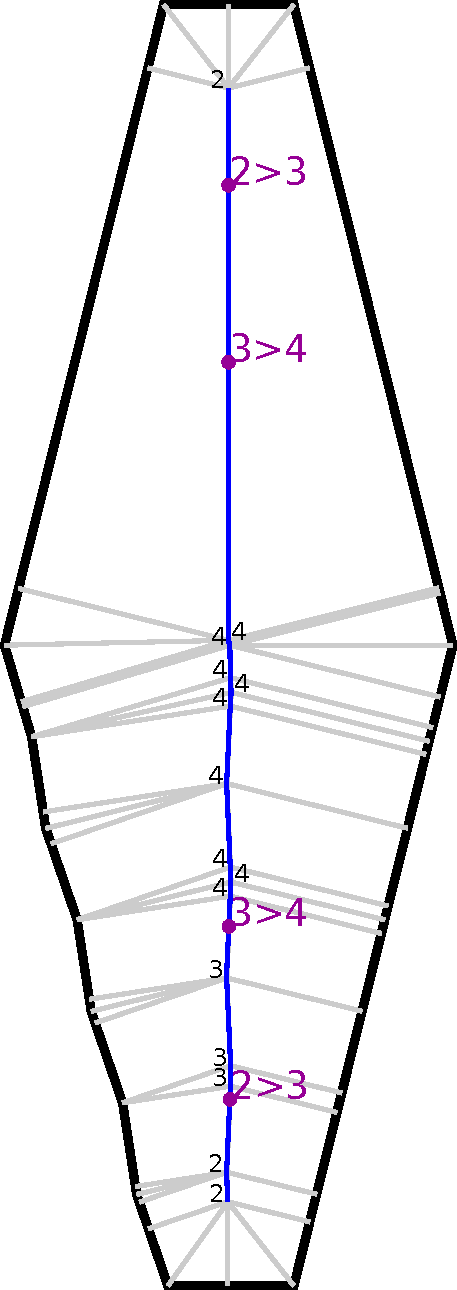
\includegraphics[width=\columnwidth]{sources/method/beading_transitioning_filtering__filtered.pdf}
\caption{Filtered anchors}\label{beading_transitioning_filtering__filtered}
\end{subfigure}
\begin{subfigure}{\figwidth}
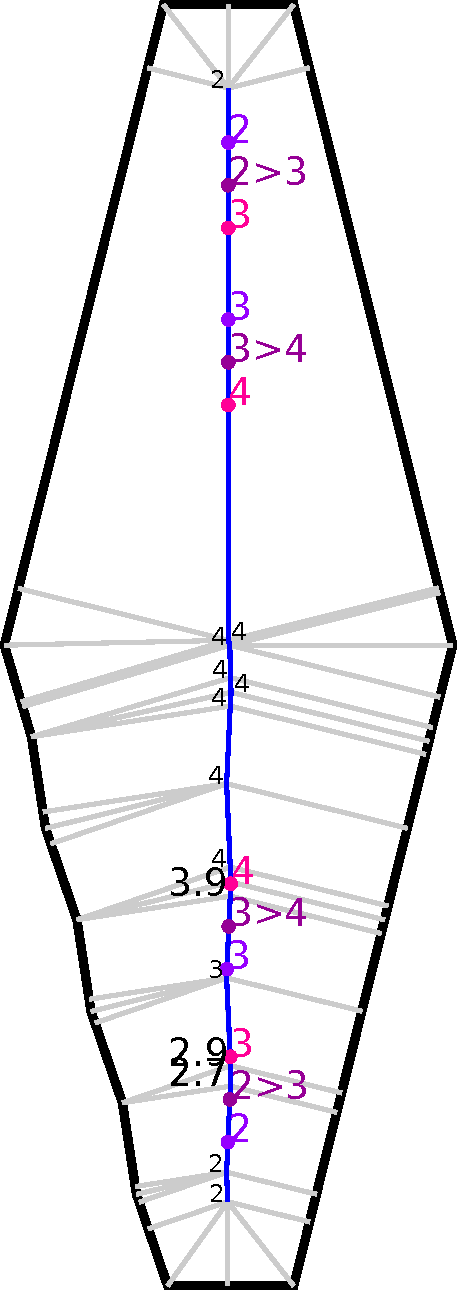
\includegraphics[width=\columnwidth]{sources/method/beading_transitioning_filtering__transition_ends.pdf}
\caption{Transition ramp ends}\label{beading_transitioning_filtering__transition_ends}
\end{subfigure}
\begin{subfigure}{\figwidth}
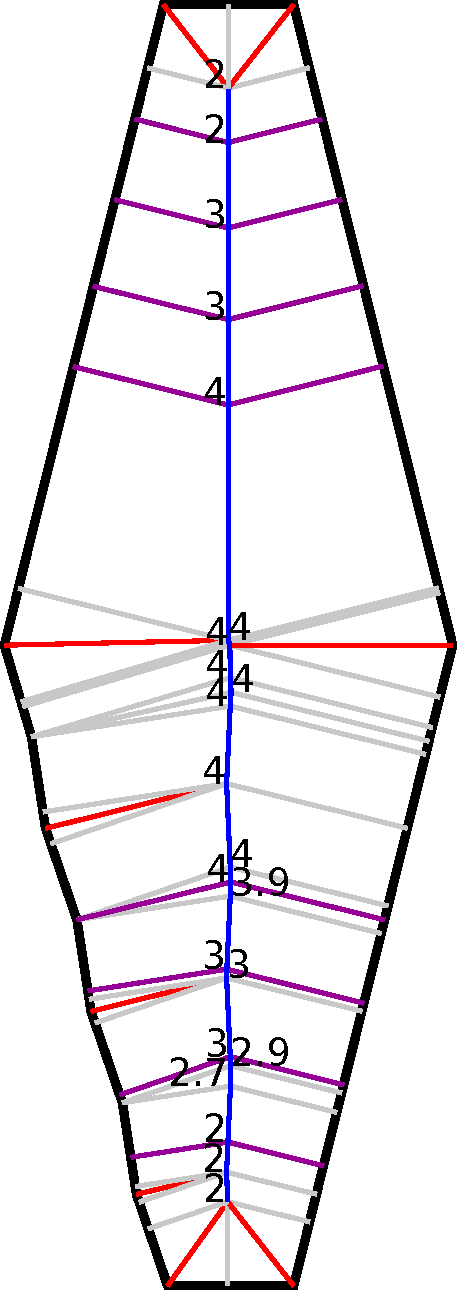
\includegraphics[width=\columnwidth]{sources/method/beading_transitioning_filtering__transitions_applied.pdf}
\caption{Radial support bones}\label{beading_transitioning_filtering__transitions_applied}
\end{subfigure}
\begin{subfigure}{.27\textwidth}
\hspace*{-.5cm}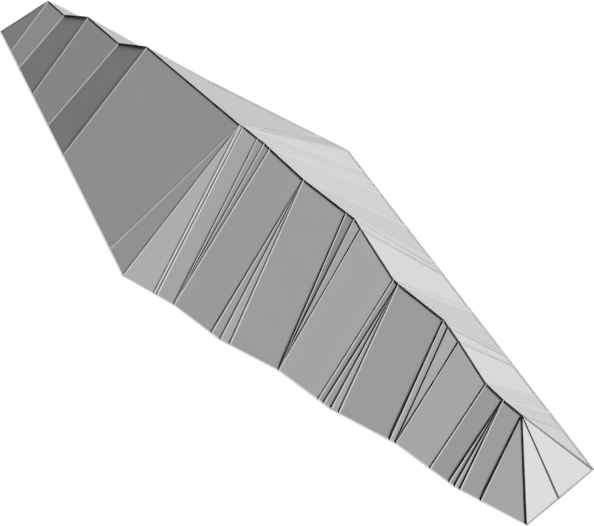
\includegraphics[width=1.2\columnwidth]{sources/method/beading_transitioning_filtering__result_uoc.png}
\caption{Result UoC}\label{beading_transitioning_filtering__result_uoc}
\end{subfigure}
\caption{
Applying bead counts and transitioning on a shape showing the difference between a simple skeleton (top) and a mirrored version with small perturbations in the outline (bottom).
Outline in black, medial axis edges in red, radial edges in grey.
\subref{beading_transitioning_filtering__bead_count} First we initialize the bead counts (black) in the marked regions (blue).
\subref{beading_transitioning_filtering__transition_mids} We then extract the anchor locations (purple) of the transitions to a different bead count should be.
\subref{beading_transitioning_filtering__filtered} We then filter out regions of constant bead count.
\subref{beading_transitioning_filtering__transition_ends} We then calculate the end locations (magenta, pink) of the transitions and modify the bead count at nodes in between to fractional values.
\subref{beading_transitioning_filtering__transitions_applied} Finally we introduce nodes at the ends and introduce radial edges (purple) as per the trapezoidation constraint.
The symmetry in the result shows that transitioning is robust against small perturbations in the outline shape.
}
\label{beading_transitioning_filtering}
\end{figure*}


\subsubsection{Flattening}
For bones which connect two nodes $v_0$ and $v_1$ with a different bead count assigned $b^*_{v_0} \neq b^*_{v_1}$ we must figure out the exact location(s $v$ where the flattening operator $f(2R(v))$ jump to a different integer.
We call these locations the \emph{transition anchor positions}.
Rather than applying the jumps to the UoC mesh we calculate the transition anchor positions and apply smoothing based on those positions, so that we modify the UoC mesh afterwards.

We introduce the function $f^{-1}(n) := \argmax_d f(d) = n$, which gives the feature diameter at which $f$ jumps from $n$ to $n+1$ beads.
%For each marked bone between $v_0$ and $v_1$ with $b^*_{v_0} \neq b^*_{v_1}$ we introduce transitions.
A smoothed transition from bead count $n$ to $n+1$ will be anchored on each location $v_x$ where $R(v_x) = f^{-1}(n)$.
We can compute the location of the anchor simply as
$$v_x = v_0 + (v_1 - v_0) \frac{ f^{-1}(n) - R(v_0) }{ R(v_1) - R(v_0) }$$
for each $n$ such that $b^*_{v_0}<n<b^*_{v_1}$.
See \cref{beading_transitioning_filtering__transition_mids}.

In order to prevent frequent oscillations in the bead count, we filter locally maximal or minimal bead count regions.
For each edge which contains a transition anchor we walk along the marked regions until we encounter another anchor.
If the other anchor is a transition in the opposite direction and the traversed distance is within some limit $d_\text{max}^\text{transition}$ we remove the transitions and set the bead counts at all nodes in the filtered region to the surrounding bead counts.
See \cref{beading_transitioning_filtering__filtered}.






\subsubsection{Smoothing}
In order to prevent discontinuities in the toolpaths around locations where the bead count changes i.e. where there is a jump in height in the UoC, we need a way to smoothly transition to a different number of beads around locations where the outline shape has a changing bead count.
See \cref{transitions}.
The length along the marked region of a transition from bead count $n$ to $n+1$ is determined by some function $t(n)$.
For our example we will use a transition length equal to the nozzle size: $t(n) = w_\text{pref}$.

A transition with length $t(n)$ will be placed somewhere covering the transition anchor position.
We require an additional function to be specified by the beading strategy: $t_0(n)$ determines the distance between the lower end of a transition from bead count $n$ to $n+1$ and the anchor point - as measured along the marked bones of the skeleton.
From that we calculate $t_1(n) = t(n) - t_0(n)$ for the distance from the anchor to the upper end of the transition.
For our example we can simply use $t_0(n) = t_1(n) = \nicefrac12 w_\text{pref}$, so that the transition ramp is centered on the anchor position.


Before we generate the transition ramps we filter out transition anchors which are positioned too close to the end of a marked region.
For each edge which contains a transition anchor we walk along the marked regions until until we have traversed a distance more than $t(n)$.
If we hit the end of a marked region and the traversed distance from the anchor point is less than the distance $t_{0}(n)$ or $t_{1}(n)$ to the transition end we dissolve the bead count region in the same manner as described above.

The generation of the transition ramps should be robust against small perturbations in the outline shape;
compare the top and bottom of \cref{beading_transitioning_filtering}.
In order to generate the lower and upper end point of the transition ramps we walk downward and upward along the marked regions from each anchor position $v$ until we have traversed the corresponding distance of $t_{0}(n)$ or $t_{1}(n)$.
If there is any node $v_x$ in between $v$ and $v_0$ or $v_1$ we assign it a fractional bead count by linear interpolation: $b^*_{v_x} = n + D(v_0, v_x)/t(n)$, where $D(.)$ is the cumulative distance measured along the marked bone(s).
See \cref{beading_transitioning_filtering__transition_ends}.
These fractional bead counts will be used in \cref{section_beading_interpolation} in a way which guarantees a similar toolpath in transitioning regions which are crossed by extra support bones for small perturbations and those which are not.

Finally we perform the mesh update by introducing nodes at the transition ends and introducing radial support bones from these new nodes to the outline as per the trapezoidation requirement.
We end up with a UoC with marked regions altered to be horizontal at integer multiples of half the nozzle width for long stretches with ramps in between.
See \cref{beading_transitioning_filtering__transitions_applied} and \subref{beading_transitioning_filtering__result_uoc}.


\begin{figure}
\centering
\setlength{\figwidth}{\columnwidth}
\begin{subfigure}{0.9\figwidth}\centering
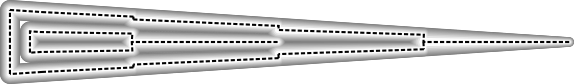
\includegraphics[width=\columnwidth]{sources/method/wedge_no_transitioning.png}
\caption{Without transitioning}
\end{subfigure}
\begin{subfigure}{0.9\figwidth}\centering
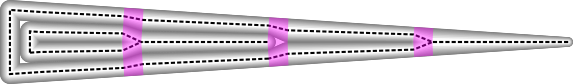
\includegraphics[width=\columnwidth]{sources/method/wedge_transitioning.png}
\caption{Transitioning}
\end{subfigure}
\caption{
Discontinuities around regions where the bead count changes are prevented by transition regions (highlighted in cyan).
}
\label{transitions}
\end{figure}














\subsection{Peripheral heights}\label{sec_peripheral_height_adjustment}
Now that we have transformed the heights in the central regions of the UoC we need to determine the heights in the rest of the shape, i.e. the periphery, and slice the resulting mesh into isocontour toolpaths.
The peripheral heights could be determined in a plethora of ways according to various beading strategies.
The ramps from the outline shape to the center might have various curves,
but for our example we use straight ramps, just like the original UoC.
See \cref{peripheral_heights}.
That means we can stretch the $R$ heights of the UoC with a multiplier depending on the height of the center in terms of bead count.


\begin{figure}\centering
\setlength{\figheight}{.2\columnwidth}
\begin{subfigure}{.55\columnwidth}\centering
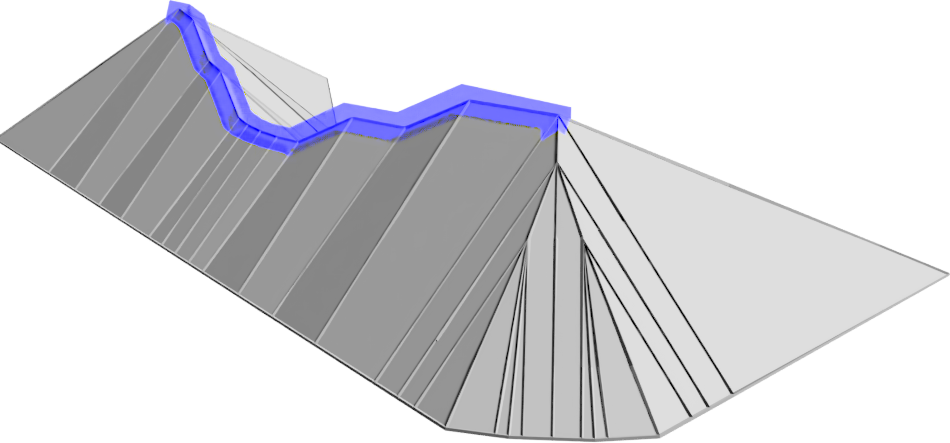
\includegraphics[height=\figheight]{sources/method/peripheral_heights_3D.png}
\caption{Surface mesh}
\end{subfigure}
\begin{subfigure}{.4\columnwidth}\centering
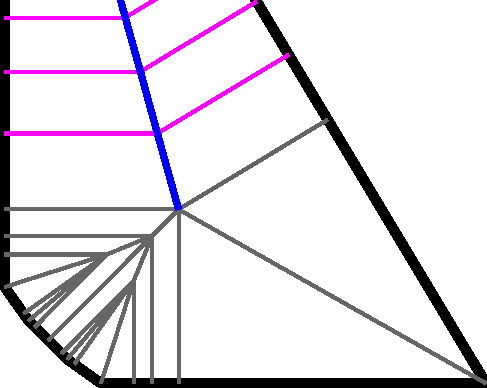
\includegraphics[height=\figheight]{sources/method/peripheral_heights.pdf}
\caption{ST}
\end{subfigure}
\caption{
Shallow corners will cause peripheral nodes for which the height should be determined based on the central node above it.
}
\label{peripheral_heights}
\end{figure}



For the purpose of generating toolpaths we only need to define the height at the locations which will be part of a slice, rather than at all locations in the periphery.
Instead of adjusting the height of peripheral mesh nodes, we determine the locations along the bones where the adjusted height coincides with a slicing height.
In this section we will show how we can define a mapping from radial distance values to the indices of slicing heights, called a \emph{beading},
how each beading is calculated for a central node
and how the beadings are propagated outward to peripheral nodes.
This helps to define an efficient slicing algorithm in \cref{sec_toolpath_extraction}.

\begin{definition}
In order to help generate these toolpath locations we associate each central node with a mapping from radial distances to bead indices, the beading $B$,
which we define as the following set:
$$
B = \left\{ d, n, \left\{ w_0 , \dots , w_{n-1} \right\}, \left\{ l_0 , \dots , l_{n-1} \right\}  \right\}
$$
where
$d = 2 R(v)$ is the diameter associated with $v$,
$n \in \mathbb{N}$ is the bead count,
$w_i$ is the bead width of the bead with index $i$ counting from the outline inward
and
$l_i$ is the radial locations which maps to the bead with index $i$.
\end{definition}

For our example we linearly map the $R$ values using a multiplication factor of $d/n$:
\begin{align*}
w_i &= d/n  \\
l_i &= d / n (i + \nicefrac12)
\end{align*}
An example beading is visualzied in the top of \cref{beading_interpolation}:
$B^V$ cover the total horizontal distance $d$ using $n=4$ beads all with the same width and radial locations $l$ evenly divided over the length $d$.


The beading information will be used in the next phase to directly generate the junctions of the toolpaths.
Note that a beading conceptually covers the whole diameter, while we only apply it along the radii;
the upper half of the beading is therefore unused.


\subsubsection{Beading interpolation}\label{section_beading_interpolation}
Central nodes which are in the middle of a transition have obtained a fractional bead count, but the definition of a beading presupposed integer numbers.
In order to generate a beading for a central node with a fractional bead count assigned we use the fractional part of the bead count to interpolate between two beadings defined on the fractional bead count rounded up and down.
Suppose we want to interpolate between two beadings $B^V$ and $B^W$, for which $n^{B^V} < n^{B^W}$.
We interpolate the diameter $d$, widths $w_i$ and locations $l_i$ for indices $i < \nicefrac12 n^{B^V}$ linearly and enforce the symmetry constraints on the upper indices.
See \cref{beading_interpolation}.
The linear interpolation enforces robustness against small perturbations in the outline shape which cause extra bones to appear in the skeleton inside of transition regions.

\iffalse
In order to create an interpolated beading $B = xB^V + (1-x) B^W$, for some $0<x<1$
we calculate:
\begin{align*}
n^{B} &= n^{B^W} \\
d^B &= x d^{B^V} + (1-x) d^{B^W} \\
w_i^{B} &= w_{n^B-i}^{B} = x w_i^{B^V} + (1-x) w_i^{B^W} \text{ for } i < \frac12 n^{B^V} \\
%  w_{frac{n}{2}^B - frac12}  = something difficult \text{ if } n \mod 2 == 1
w_i^{B} &= w_i^{B^W} \text{ otherwise}\\
l_i^{B} &= 
\begin{cases} 
x l_i^{B^V} + (1-x) l_i^{B^W} & \text{ for } i < \frac12 (n^{B^V} - 1) \\
d^B - x l_{i-n^{B^W}+n^{B^V}}^{B^V} + (1-x) l_i^{B^W} & \text{ for } i > n^B - 1 - \frac12 (n^{B^V} - 1) \\
\frac12 d^B  & \text{ if $n^B$ is odd and } i = (n^B - 1) / 2 \\
l_i^{B^W} - l_{n^{B^V}-1}^{B^W} + l_{n^{B^V}-1}^B & \text{ otherwise}
\end{cases}
\end{align*}
\fi

\begin{figure}
\centering
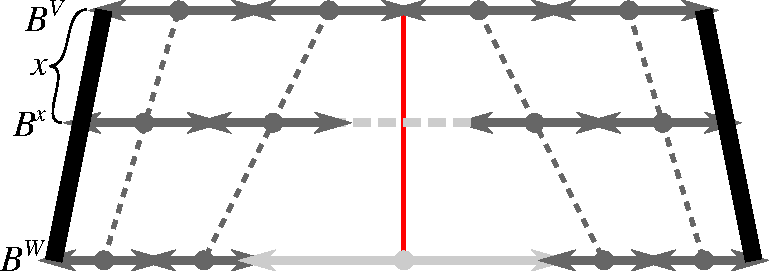
\includegraphics[width=.8\columnwidth]{sources/method/beading_interpolation_v2.pdf}
\caption{
Interpolation between two beadings $B^V$ and $B^W$ with a ratio $x$ results in a beading $B^x$.
Distances between the thick black lines constitute diameters $d$,
the toolpath locations are visualized as dots,
the widths are visualized as bidirection arrows
and the middle is highlighted in red.
}
\label{beading_interpolation}
\end{figure}


\subsubsection{Beading propagation}\label{section_beading_conflicts}
The beading information associated with the central nodes is then propagated outward throughout the whole mesh.
However, beading conflicts can arise where a marked bone has unmarked upward edges attached to them, since beading will also be propagated down from the local maxima or other higher marked regions.
See \cref{beading_conflict_problem}.
In such a case we interpolate between the lower beading and the beading propagated from above,
starting from the lower marked node and ending at a distance $t_\text{beading}$ upward.
At the nodes in between we will apply the interpolation between the two beadings and propagate the interpolated beading outward from those nodes.
This interpolation is performed during the beading propagation algorithm.


\begin{figure}\centering
\setlength{\figheight}{.2\columnwidth}
\begin{subfigure}{.45\columnwidth}\centering
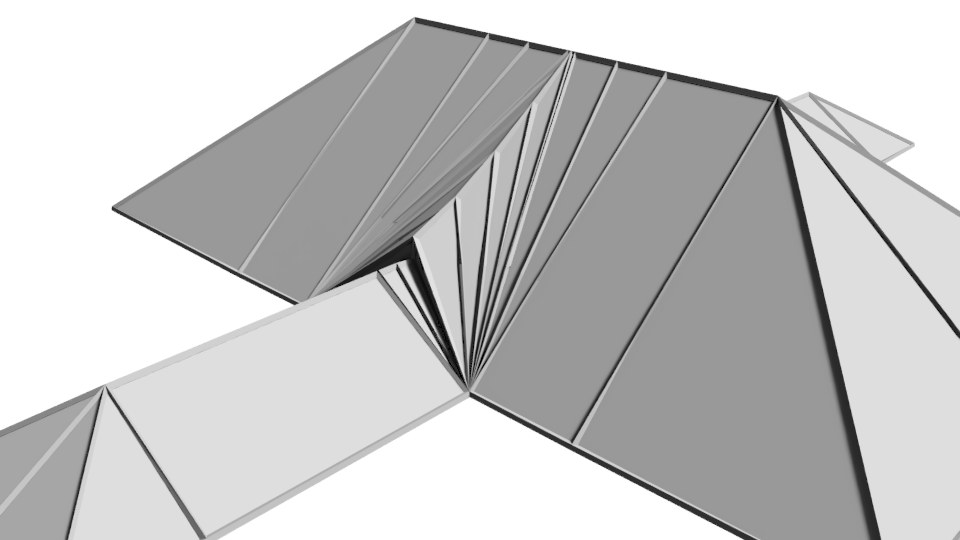
\includegraphics[width=\columnwidth]{sources/method/beading_conflict_3D.png}
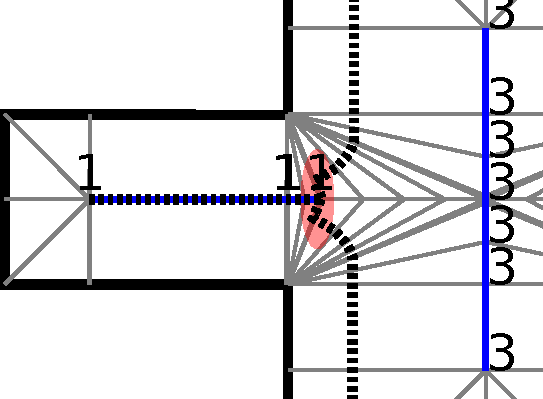
\includegraphics[height=\figheight]{sources/method/beading_conflict.pdf}
\caption{Beading conflict}\label{beading_conflict}
\end{subfigure}
\begin{subfigure}{.45\columnwidth}\centering
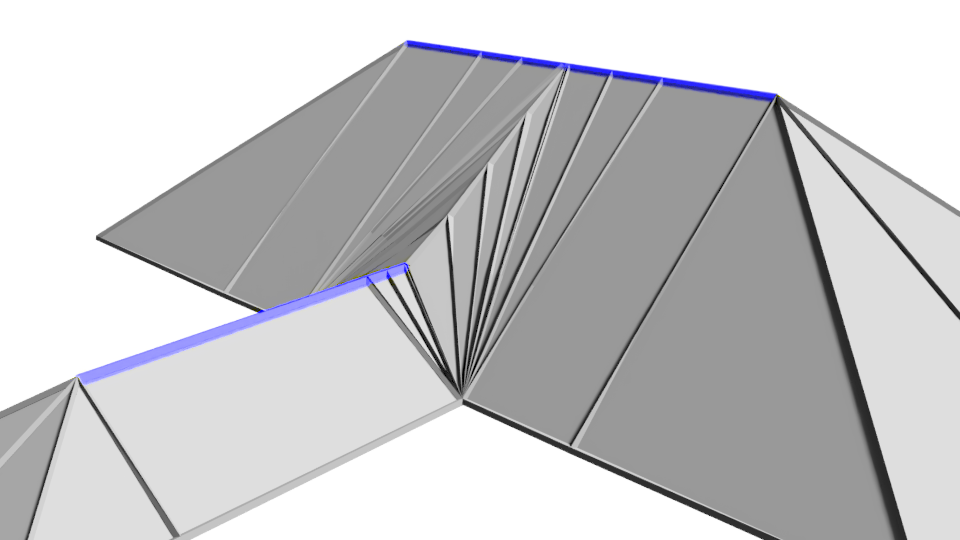
\includegraphics[width=\columnwidth]{sources/method/beading_conflict_solved_3D.png}
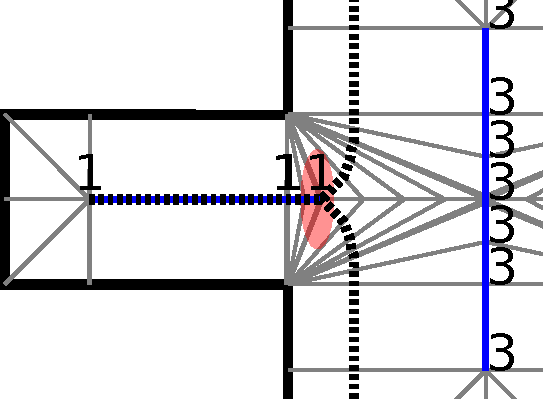
\includegraphics[height=\figheight]{sources/method/beading_conflict_solved.pdf}
\caption{Conflict resolution}\label{beading_conflict_solved}
\end{subfigure}
\caption{
\subref{beading_conflict} The beading propagated from above conflicts with the beading below.
\subref{beading_conflict_solved} The beading conflict is resolved by gradually interpolating between the two beadings.
The ramp to the upper ridge doesn't line up with the lower ridge, which means that
the toolpaths (dashed) resulting from the beading propagated from above doesn't align with the beading from the thin outline feature (highlighted in red).
}
\label{beading_conflict_problem}
\end{figure}

After each marked node is assigned a beading by the beading strategy, we propagate the beadings outward to all nodes in the ST.
The beading propagation is performed in two stages: an upward and downward stage.
%First we sort all upward half-edges on the radial distance of their destination node, so that we can efficiently flood fill the beading information.
In the upward phase we walk from each marked node upward along unmarked edges and map each node encountered to a pair consisting of the traversed distance and the bottom source beading.
In the downward phase we walk from each marked node downward along unmarked edges and map each node to a pair consisting of the traversed distance and the upper source beading -
however, if we encounter a node which was already mapped to an upward propagated beading we employ the interpolation scheme described above in order to define the beading, which is then further propagated downward.
This is implemented in a flood-fill fashion: see \cref{alg_beading_propagation}.

\begin{algorithm}
\caption{Beading propagation}
\label{alg_beading_propagation}
\begin{algorithmic}
\ForAll{$v \in$ nodes}
	\If {marked($v$)} $\text{map}[v] = (0, B(b^*_v, 2 R(v)))$ \EndIf
\EndFor
\ForAll{$e \in$ edges}
	\If {$R(v_0^e) < R(v_1^e)$}
		% \State 
		upwardEdges.add($e$)
	\EndIf
\EndFor
\State upwardEdges.sort($\uplambda e_1 e_2 . R(v_1^{e_1}) < R(v_1^{e_2})$) \Comment {low to high $v_1$}
\ForAll{$e \in$ upwardEdges} \Comment{upward phase}
	\If {$\text{map}[v_0^e] \land \neg \text{map}[v_1^e$]}
    		\State $(d, B) = \text{map}[v_0^e]$
    		\State $\text{map}[v_1^e] \leftarrow (d + |v_1^e - v_0^e|, B)$
	\EndIf
\EndFor
\ForAll{$e \in$ reverse(upwardEdges)} \Comment{downward phase}
	\If {$\text{map}[v_1^e]$}
    		\State $(d, B) \leftarrow \text{map}[v_1^e]$
    		% d + |v_1^e - v_0^e|
    		\If {$\text{map}[v_0^e]$}
    			\State $(d_0, B_0) = \text{map}[v_0^e]$
    			\State $B \leftarrow \text{interpolate}(\min(1, d_0 /  t_\text{beading}), B_0, B)$
    		\EndIf
    		\State $\text{map}[v_1^e] \leftarrow (0, B)$
	\EndIf
\EndFor
\end{algorithmic}
\end{algorithm}
















\subsection{Toolpath extraction}\label{sec_toolpath_extraction}
Now that each node has a beading associated with it we can apply the beading to generate the junctions of the toolpaths.
For each upward half-edge $e$ we generate each junction $J$ based on the beading $B = B^{v_1^e}$:
\begin{align*}
J &= \{ v, w, i \} \\ 
v &= v_1^e + (v_0^e - v_1^e) \frac{R(v_1^e) - l_i^B}{R(v_1^e) - R(v_0^e)} \\ 
w &= w_i^B
% \\ i^J &= i
\end{align*}
for any $i$ for which $R(v_0^e) < l_i^B \leq R(v_1^e)$.
See \cref{junction_placement}.
We store all junctions of a segment in a mapping from edge to a list of junctions.


\begin{figure}
\centering
\setlength{\figheight}{.29\columnwidth}
\begin{subfigure}{0.14\columnwidth}\centering
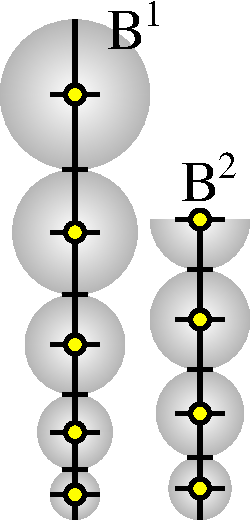
\includegraphics[height=\figheight]{sources/method/trapezoid_beading_beading.pdf}
\caption{Beadings}\label{trapezoid_beading_beading}
\end{subfigure}
\begin{subfigure}{0.5\columnwidth}\centering
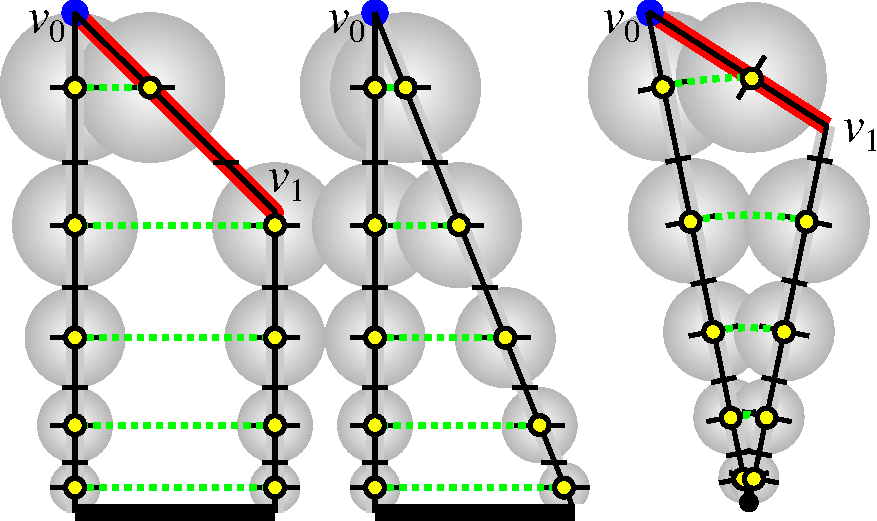
\includegraphics[height=\figheight]{sources/method/trapezoid_beading_propagated.pdf}
\caption{Single beading propagated to all nodes}\label{trapezoid_beading_propagated}
\end{subfigure}
\begin{subfigure}{0.34\columnwidth}\centering
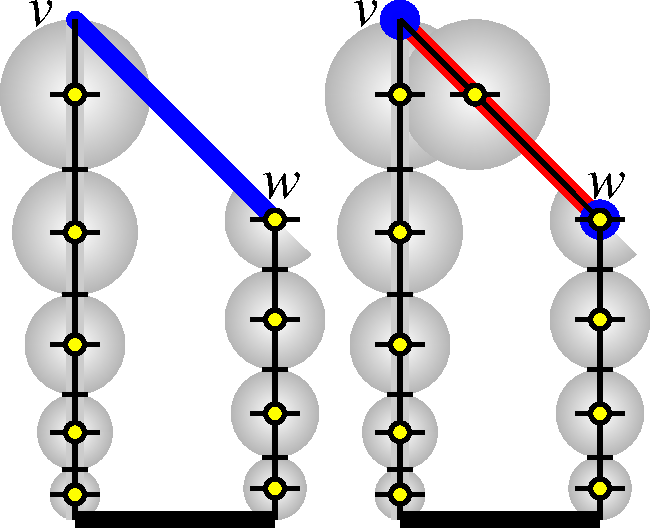
\includegraphics[height=\figheight]{sources/method/trapezoid_beading_separate.pdf}
\caption{Separate beadings at either top node}\label{trapezoid_beading_separate}
\end{subfigure}
\caption{
Applying beadings togenerate junctions along trapezoids.
\subref{trapezoid_beading_beading} shows half of the locations $l_i$ and widths $w_i$ of two arbitrary different beadings.
\subref{trapezoid_beading_propagated} shows the application of $B^1$ to the various types of trapezoid.
\subref{trapezoid_beading_separate} shows how a trapezoid with a marked edge will have two different beadings assigned, which will generate their respective junctions along the support bones.
No junctions will be generated along marked bones.
Wide black lines are outline segments, marked nodes and bones in blue, the junctions in yellow and green wavefronts of equidistant radial distance at $R = l_i$.
}
\label{junction_placement}
\end{figure}


We then generate bead segments for each trapezoid by connecting together the junctions of the same index.
See \cref{segment_generation}.
If the amount of junctions on both sides of the trapezoid is not the same then this trapezoid is in a transition and we leave one inner junction unconnected.
If a central edge has both nodes with an odd bead count assigned to it $b^* \bmod 2 = 1 $ we should prevent the algorithm from generating the center segment from both trapezoids.
We therefore use some arbitrary condition to decide which one of the two to include based on the ordering of the coordinates of $v_0$ and $v_1$.

Each of the trapezoids is connecting to a single outline polygon.
By traversing the trapezoids in the domain of each outline polygon in order we can efficiently connect all segments into polylines.
See \cref{segment_generation}.
In a final step we connect the ends of polylines together, so that the final toolpaths contain both polygons and polylines.

\begin{figure}
\centering
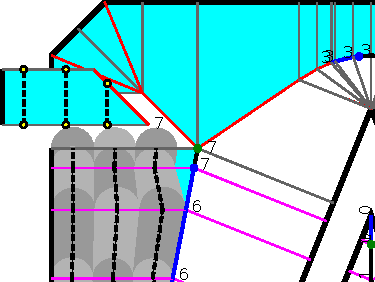
\includegraphics[width=.5\columnwidth]{sources/method/segment_generation.pdf}
\caption{
Generating toolpaths on a part of the test outline shape which is fully shown in \cref{shape_decomposition_domains}.
Each edge is assigned toolpath junctions (yellow) which are connected together as shown in the singled out trapezoid.
By following the trapezoids along the domain (cyan) of a single outline polygon,
the segments can efficiently be connected into existing polyline toolpaths (light and dark gray).
}
\label{segment_generation}
\end{figure}


Around the transition locations and around nodes with odd bead count and more than two marked edges attached there will be intersections in the toolpaths.
Such intersections cause overextrusion because the nozzle passes the location multiple times.
In order to reduce the amount of overextrusion of a polyline ending in a junction $J$ we therefore remove part of the polyline paths up to the intersection by a distance of $w^J d_\text{max}^\text{intersection}$, where $d_\text{max}$ is some ration between $0$ and $1$.
We do this for all polylines until only two outward toolpath segments remain, which constitute a single pass over the junction.
See \cref{polyline_reduction}.


\begin{figure}
\centering
\setlength{\figwidth}{\columnwidth}
\begin{subfigure}{0.45\figwidth}\centering
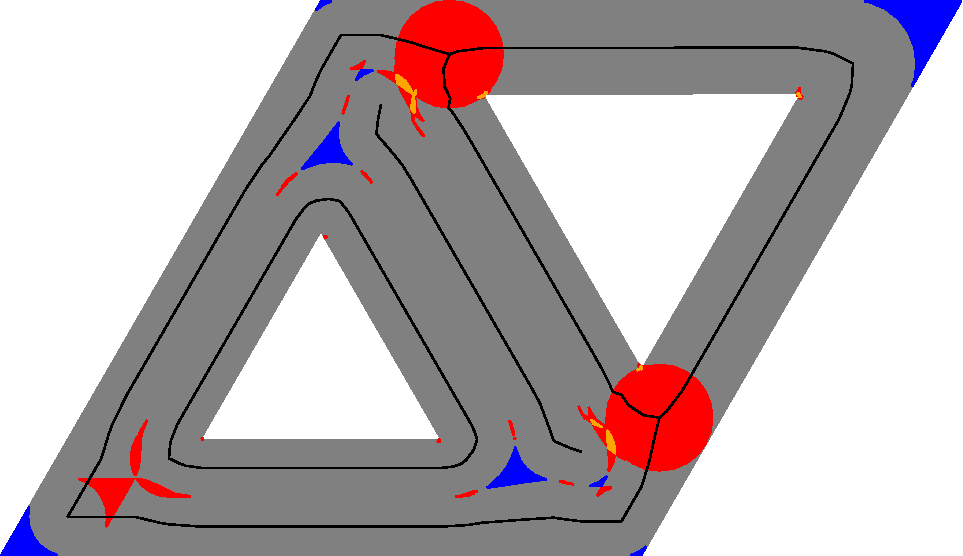
\includegraphics[width=\columnwidth]{sources/method/polyline_reduction_unreduced.pdf}
\caption{No reduction}
\end{subfigure}
\begin{subfigure}{0.45\figwidth}\centering
\includegraphics[width=\columnwidth]{sources/method/polyline_reduction_reduced.pdf}
\caption{Reduction}
\end{subfigure}
\caption{
Reducing polyline toolpaths away from intersections in order to prevent overextrusion.
Toolpath locations in black, underextrusion in blue, overextrusion in red and orange and normal extrusion in grey.
Intersections result in overextrusion, so we remove parts of the polylines at intersections.
}
\label{polyline_reduction}
\end{figure}



























































